\chapter{The genomics of the Slavic migration period, Early Middle Ages and their links to the present day}
\label{chapterlabel5}

\section{Introduction}

The Slavic peoples originated as a diverse network of tribal societies who lived in Central and Eastern Europe from the first Millennia AD \cite{barford2001early} and whose origin, although disputed, is thought to be Polesia (a marshy forested area straddling Poland, Belarus, Russia and Ukraine) \cite{fouracre1995new}. Although various Roman and Greek sources refer to Slavs as \textit{Veneti} and \textit{Spori} as early as the 1st and 2nd centuries AD, the term `Slavs' was first used in writing by Roman bureaucrat Jordanes at the beginning of the 6th century after their attack on the Byzantine empire \cite{curta2006southeastern}. This era, known by historians as The Migration Period, was a period of European history, roughly between 375-568 AD after the fall of the Roman Empire \cite{halsall2007barbarian}, characterised by the large-scale movement of various peoples. The Migration Period began with the Huns moving into Eastern Europe at the end of the 4th Century, occupying an area including present-day Hungary and Romania. During the 5th century, various Germanic groups invaded and established a homeland across parts of the Western Roman Empire. This was followed by the expansion of Slavic populations into regions of low population density in the sixth century.

Across the next two centuries, these peoples had settled across large parts of Europe (Fig. \ref{fig:Slavic_tribes}). In particular, the Early Slavs had expanded southwards into the Balkans and Alps \cite{barford2001early, brather2008archaologie, geary2003myth,gojda1991ancient}. It has been proposed that these migrations were key to forming the foundations of present-day Slavic (speaking) nations \cite{barford2001early}.  

By the beginning of the 12th century, Slavs constituted a large part of a number of many medieval Christian states across Europe. As from this time period, Slavs could be broadly split up in three groups: the eastern Slavs as part of the Kievan Rus', southern Slavs in the Bulgarian Empire, the Principality of Serbia, Kingdom of Croatia and the Banate of Bosnia, and western Slavs in the Principality of Nitra, Great Moravia, the duchy of Bohemia and the Kingdom and Poland. In addition, Slavic settlement also occurred in the Eastern Alps; Slovenia, large parts of present-day Austria and Friul. 

\begin{figure}[htp]
    \centering
    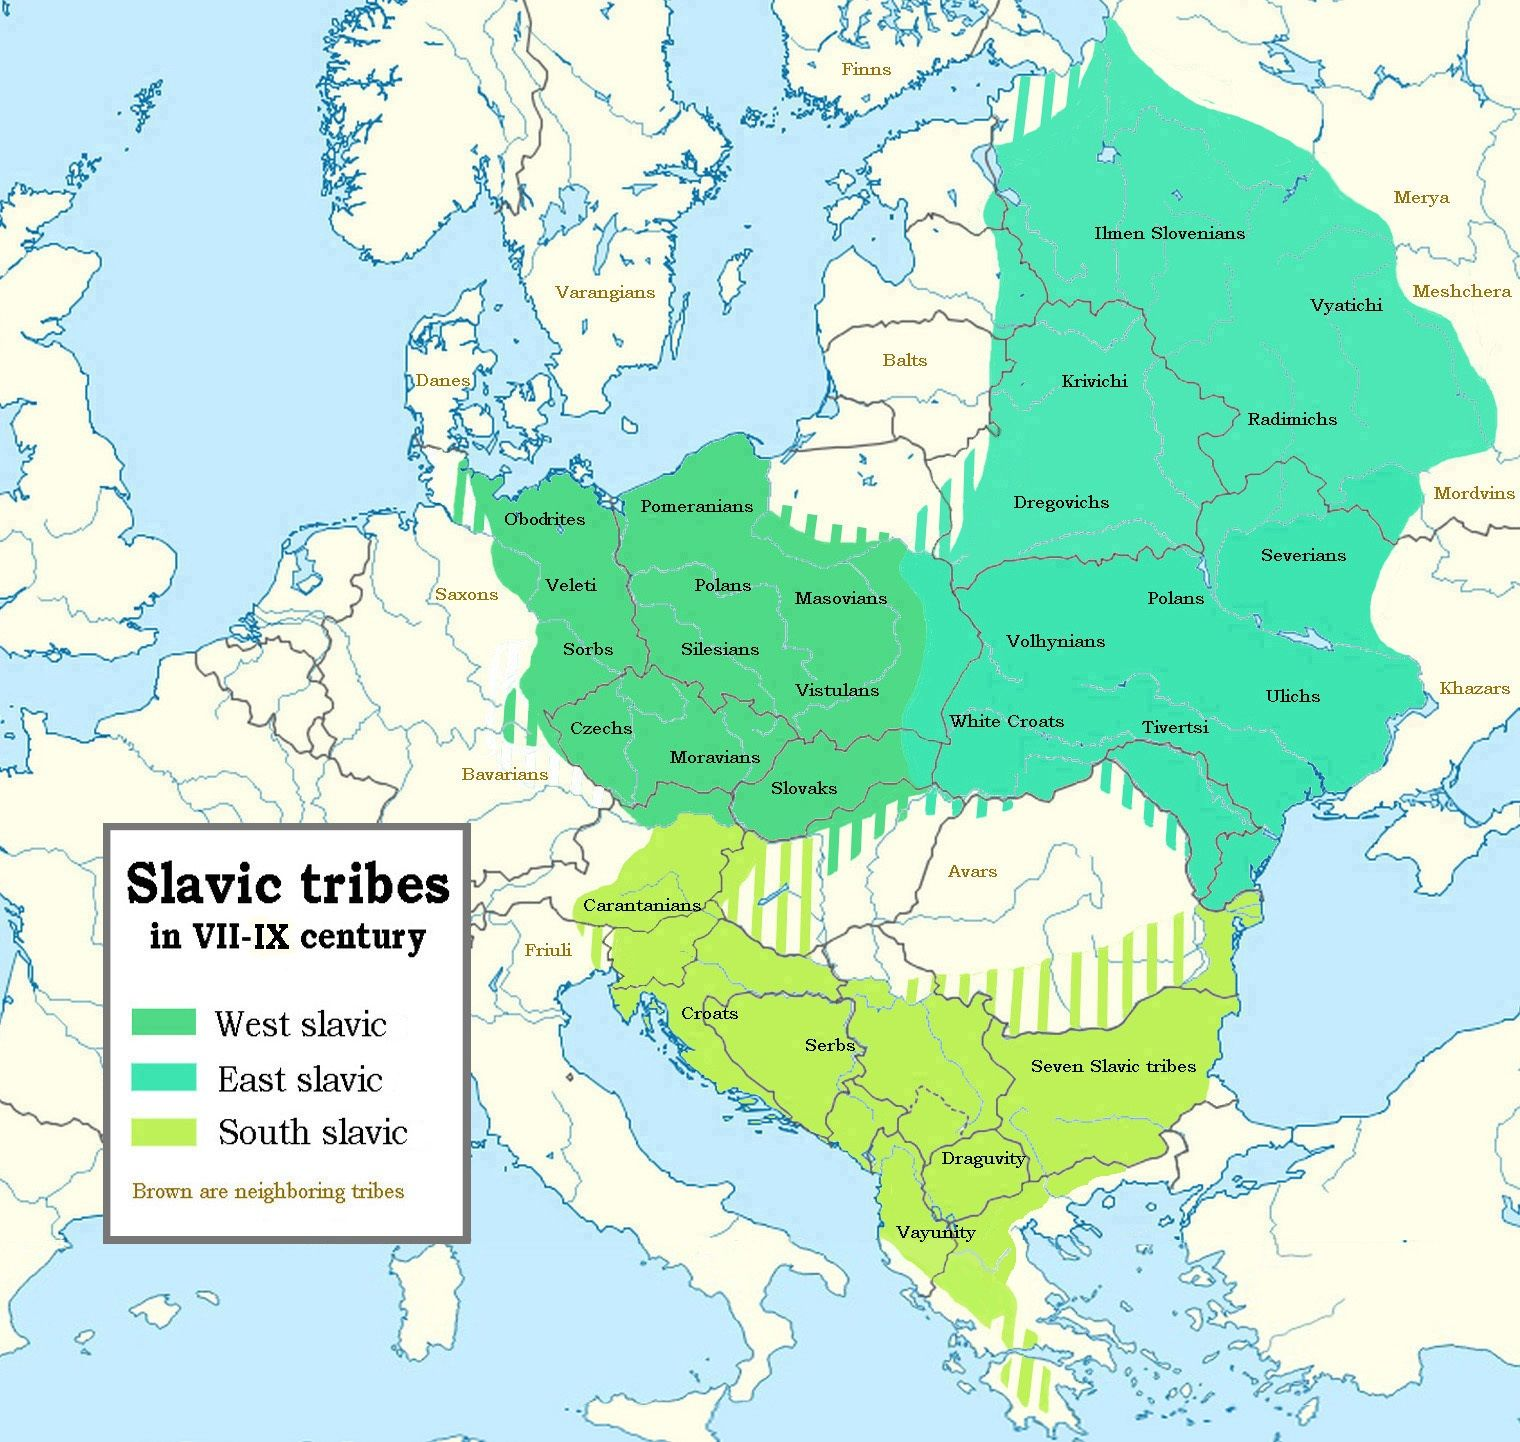
\includegraphics[width=1.0\textwidth]{../images/chapter5/Slavic_tribes_in_the_7th_to_9th_century.jpg}
    \caption{Slavic tribes from the 7th to 9th centuries AD in Europe. Source: (\url{https://commons.wikimedia.org/wiki/File:Slavic_tribes_in_the_7th_to_9th_century.jpg})}
    \label{fig:Slavic_tribes}
\end{figure}

 Today 315 million people speak Slavic languages and linguistic evidence suggests that they can be broadly split into these three broad groups; western Slavs (Poles, Czechs and Slovaks), eastern Slavs (Ukrainians, Belarusians and Russians) and southern Slavs (Croatians, Bulgarians, Slovenians, Bosnians, Macedonians, Montenegrins and Serbians) \cite{sussex2006slavic}. 

The history of the Slavic peoples can be artificially be split into three periods: Migration Period ($\sim$375AD - $\sim$568AD), Early Middle Ages/High Middle Ages ($\sim$600AD - $\sim$1250AD) and present-day. Several previous studies have investigated the genetics of the transitions between these periods. Juras et al (2014) used uni-parental mtDNA markers from ancient DNA samples from Poland to show continuity between both Roman Iron Age period (200 BC – 500 AD) and Medieval Age (1000–1400AD) with present-day Poles, Czechs and Slovaks \cite{Juras2014}. However, whilst informative about sex-biased migrations, uniparental markers carry only a fraction of the information that autosomal markers do, and therefore may provide misleading or incomplete information about the relationship between  samples \cite{Shaw16122, malinsky2018whole}, especially when admixture is prevalent (although see \cite{Mitochondrial}). For example, it is know that mtDNA and nuclear DNA may have different evolutionary histories and thus display discordant phylogenetic trees \cite{posth2017deeply}. 

Kushniarevich et al (2015) \cite{Kushniarevich23015} combined results from mtDNA, non-recombining Y and autosomal DNA to investigate the population structure of a wide range of present-day Balto-Slavic populations. They proposed that incoming Slavic speakers admixed with peoples in the regions they occupied during the Migration Period. 

More recently, Macháček et al (2021) \cite{MACHACEK2021105333} analysed a cattle rib from Lány, Czechia, dated to approximately 600AD, that is inscribed with Germanic runes. The bone was found in a location where Slavs were thought to have arrived at the end of the Migration Period, after the Germanic tribes had disappeared and the use of a Slavic language is historically confirmed as of the 9th century. However, whether there was early genetic contact as well is yet to be determined. 

Several studies into present-day Slavic populations have detected signatures of admixture from East-Asia \cite{Hellenthal2014, pankratov2016east, MOSAIC_2019, maliarchuk2008origin, qin2015quantitating}. Whether or not these signals can be observed in ancient individuals is yet to be seen and could further refine the admixture date. For example, different admixture dates in different Slavic populations may reveal structure among present-day Slavs. 

Finally, several studies have used haplotype-based methods to explore the structure of present-day Slavic populations. Ralph and Coop \cite{RalphCoop2013} compared regions of IBD matching  across different European populations. They found a relatively high degree of IBD sharing among pairs of individuals from Eastern Europe, suggestive of expansion from a smaller, common source population. This expansion was tentatively estimated to between 0-1000AD. Consistent with estimates of a small population size, Hellenthal et al (2014) \cite{Hellenthal2014} inferred an excess of among Eastern European individuals and an admixture event, albeit with a more constrained admixture date of 440 - 1080 CE. However, this could also be interpreted in terms of a small effective population size \cite{al2019estimating, ringbauer2017inferring}. Salter-Townshend and Myers (2019) also identified admixture in the Chuvash people between east Europeans and east Asians approximately 1224 CE \cite{MOSAIC_2019}.

In this chapter, I will analyse 17 new medium to high coverage whole ancient genomes from Czech Republic, spanning from the Migration Period to Early Middle Ages (384-950 AD). These are, to my knowledge, the first high-coverage whole ancient-genomes from this period. I will merge the newly sequenced samples with reference data from other ancient individuals and a large reference set of relevant present-day European individuals in order to understand their ancestry in the context of both present-day and ancient samples. In particular, I am interested in considering the following questions:

\begin{enumerate}
\item Do the labels "Migration Period" and "Early Middle Ages" make sense from a genetic standpoint? Is there evidence of genetic change between Migration period and Early Middle Ages in the area of present-day Czech Republic). 
\item Is it possible to use these samples to reject a null-model of continuity between the Migration Era and Early Middle Ages?
\item How are present-day Slavic speakers structured, and do the different ancient Slavic samples have different affinities to different present-day Slavic language groups?
\end{enumerate}


\section{Methods}

\subsection{Description of samples}

Whole-genome sequence data were generated from 17 ancient individuals (Table \ref{tab:AncientSamples}). Five samples from Líbivá date to the Migration Period (348 AD - 504 AD), while the other 12 samples from Pohansko date to the later Early Middle Ages (724 AD - 995 AD).

\begin{table}
\centering
\begin{tabular}[t]{llrlr}
\toprule
Code & Site & Date (AD) & Period & Coverage\\
\midrule
LIB11 & Břeclav – Líbivá & 741.5 & Early Middle Ages & 5.3\\
LIB12 & Břeclav – Líbivá & 475.5 & Migration period & 6.8\\
LIB2 & Břeclav – Líbivá & 495.0 & Migration period & 6.4\\
LIB3 & Břeclav – Líbivá & 509.0 & Migration period & 5.3\\
LIB4 & Břeclav – Líbivá & 472.5 & Migration period & 6.5\\
\addlinespace
LIB5 & Břeclav – Líbivá & 348.0 & Migration period & 7.3\\
LIB7 & Břeclav – Líbivá & 830.5 & Early Middle Ages & 5.6\\
POH11 & Pohansko – Lesní školka & 783.0 & Early Middle Ages & 5.0\\
POH13 & Pohansko – Lesní školka & 879.5 & Early Middle Ages & 6.0\\
POH27 & Pohansko – Jizní Předhradí & 783.0 & Early Middle Ages & 5.9\\
\addlinespace
POH28 & Pohansko – Jizní Předhradí & 822.5 & Early Middle Ages & 5.6\\
POH36 & Pohansko – Jizní Předhradí & 880.5 & Early Middle Ages & 5.5\\
POH39 & Pohansko – Jizní Předhradí & 866.4 & Early Middle Ages & 5.3\\
POH3 & Pohansko – Lesní hrúd & 956.5 & Early Middle Ages & 5.4\\
POH40 & Pohansko – Lesní školka & 950.5 & Early Middle Ages & 5.5\\
\addlinespace
POH41 & Pohansko – Lesní školka & 875.5 & Early Middle Ages & 5.2\\
POH44 & Pohansko – Pohřebištĕ U Kostela & NA & Early Middle Ages & 5.3\\
\bottomrule
\end{tabular}
\caption{Information on newly sequenced ancient samples. Date (AD) estimated from radiocarbon dating. `Migration' corresponds to Migration Period and `EMA' corresponds to Early Middle Ages. Coverage calculated as the mean depth across all 77,213,942 genome-wide SNPs where genotypes were called at.}
\label{tab:AncientSamples}
\end{table}

The Migration Period and Early Middle Age samples were categorised based upon the style of pottery found in the burial grounds (Z. Hofmanová, personal communication).  


\subsection{Ancient DNA processing} \label{AncientDNAprocessing}

I merged the 17 newly sequenced individuals with the ancient literature samples given in section \ref{section:AncientReferenceDataset}, resulting in a total of 959 ancient individuals with genotype likelihoods at 77,213,942 genome-wide autosomal SNPs. 

I followed the GLIMPSE \cite{rubinacci2021efficient} imputation and phasing pipeline (\url{https://odelaneau.github.io/GLIMPSE/tutorial_b38.html}) to generate genotype probabilities and phased genotypes for each individual. For the reference panel, I used the 30x 1000 genomes dataset \cite{byrska2021high}, described in Appendix section \ref{section:1000genomes}.  

\subsection{Present-day DNA processing} \label{PresentdayDNAprocessing}

I  merged the newly sequenced and published ancient samples with the MS-POBI-HellBus dataset, described in detail in Appendix section \ref{section:MSPOBIHellBus}, chosen because it contains a high number of relevant samples from central and eastern Europe. I removed samples from Australia, New Zealand and USA.

The present-day and ancient samples were phased separately, as GLIMPSE is designed for sequence-level density of data, and the present-day samples were genotyped on a low-density genotyping array. Therefore, I phased the present-day samples using shapeit4 \cite{delaneau2018integrative} using default parameters and the supplied genetic map. I note that phasing the datasets separately may reduce power to compare ancient and present-day samples. 

The present-day and ancient samples described in section \ref{AncientDNAprocessing} were merged and converted to ChromoPainter format.

\subsection{plink PCA}

I performed a PCA on the pre-imputation genotypes using plink2 \cite{chang2015second}. I chose to use plink2 because recent studies have shown it is substantially better at dealing with samples containing variable amounts of missing data than other methods such as smartPCA \cite{AlbrechtsenPCAmissingness}.

I retained only the 500,000 markers with the lowest amount of missingness. I then LD-pruned the resulting SNPs using the settings \texttt{--maf 0.01} and \texttt{--indep-pairwise 50 5 0.2} and performed PCA using plink2 under default settings. 

\subsection{Allele-frequency based tests}

I used Admixtools \cite{Patterson2012}, implemented in Admixr R library \cite{admixrpetr2019} to perform  different F-statistics.

\subsection{ChromoPainter and fineSTRUCTURE analysis}

The merged data described in sections \ref{AncientDNAprocessing} and \ref{PresentdayDNAprocessing} contained a total of 959 ancient and 14,795 present-day samples genotyped at 477,417 autosomal bi-allelic SNPs.

I first selected all ancient samples above 2x coverage and performed an `all-v-all' painting where each haplotype was compared to all other haplotypes in turn, hereafter referred to as `ancient' painting. I chose to remove samples with $<$2x coverage because all new samples analysed here had at least 5x coverage, and my previous work indicated little difference in ChromoPainter results among samples $>$2x coverage (Chapter 2 section \ref{sec:ChromoPainterChap2}). 

I also performed an `all-v-all' painting of the 17 newly sequenced samples and the present-day populations given in table \ref{table:present-day_inds_painting}, hereafter referred to as `present-day painting'.


The fineSTRUCTURE \cite{Lawson2012} clustering and tree building algorithm was applied to the ChromoPainter output for both the `present-day' and `ancient' paintings, in each case using 2,000,000 MCMC iterations after 1,000,000 iterations of ``burn-in''. I then ran the tree-building mode (-m T) with 100,000 additional hill-climbing steps before tree building,

Tree figures, coancestry matrix figures and principle component plots were generated using the fineSTRUCTURE R library \url{(https://people.maths.bris.ac.uk/~madjl/finestructure/FinestructureRcode.zip)}.

\begin{table}
\centering
\begin{tabular}[t]{lc}
\toprule
Population & \thead{Number of\\ Individuals}\\
\midrule
HB:tsi & 98\\
HB:spanish & 34\\
HB:german & 30\\
HB:french & 28\\
HB:greek & 20\\
HB:croatian & 19\\
HB:hungarian & 19\\
HB:norwegian & 18\\
HB:southitalian & 18\\
HB:polish & 17\\
HB:romanian & 16\\
HB:mordovian & 15\\
HB:cypriot & 12\\
HB:northitalian & 12\\
HB:lithuanian & 10\\
HB:siciliane & 10\\
HB:westsicilian & 10\\
HB:tuscan & 8\\
HB:irish & 7\\
HB:scottish & 6\\
HB:germanyaustria & 4\\
HB:welsh & 4\\
\bottomrule
\end{tabular}
\caption{Name of population and number of samples used in the present-day ChromoPainter analysis}
\label{table:present-day_inds_painting}
\end{table}

\subsection{SOURCEFIND ancestry proportion analysis}

I used SOURCEFIND \cite{Chacon-Duque2018} to infer the proportions of ancestry by which each target (e.g.\ ancient) individual is most related to a set of surrogate ancient populations. Each of the 47 clusters of ancient samples inferred by fineSTRUCTURE was analysed in turn, using the other 46 clusters to act as surrogates.    

Each cluster was run across three independent MCMC runs, using 50,000 burn-in iterations, 500,000 main iterations, and thinning every 5 iterations All three MCMC runs were then combined to form an MCMC list using the coda R libary \cite{oro22547} and \texttt{mcmc} function to jointly estimate ancestry proportions and empirical credible intervals for each target population. 

\subsection{MOSAIC admixture analysis}

I inferred admixture events, dates and proportions using  MOSAIC \cite{MOSAIC_2019}, performing two different analyses that mimicked the two ChromoPainter ``ancient'' and ``present-day'' paintings described above. In particular I tested each of the 5 fineSTRUCTURE clusters containing the 17 newly sequenced individuals using as surrogates: (i) 46 other fineSTRUCTURE clusters containing ancient individuals (i.e.\ from the ``ancient'' painting results) or (ii) only the 5 other Slavic ancient populations plus 49 present-day populations in Table \ref{tab:MOSAIC_pops_slav}. I assumed each target population could be formed as a mixture of both two and three admixing sources, with all other parameters left as default. 

I then performed a `present-day surrogates' analysis using a select group of present-day populations \ref{tab:MOSAIC_pops_slav} and all ancient Slavic samples. I analysed each population in turn using all other populations as surrogates.  

MOSAIC was run using default settings and the following sets of populations as targets and the following sets as surrogates. I formed each target as a mixture of both 2 and 3 mixing sources, with all other parameters left as default. Upper and lower quantiles for admixture dates were estimated using a bootstrap procedure. Other than changing the number of mixing sources, all other parameters were left as default.

\begin{table}
\small
\centering
\begin{tabular}[t]{lr}
\toprule
Population & \thead{Number of \\Individuals}\\
\midrule
HB:han & 34\\
HB:bulgarian & 31\\
HB:japanese & 28\\
HB:sardinian & 28\\
HB:russian & 25\\
HB:yakut & 25\\
HB:greek & 20\\
HB:ukrainian & 20\\
HB:croatian & 19\\
HB:hungarian & 19\\
HB:mongolian & 19\\
HB:southitalian & 18\\
HB:chuvash & 17\\
HB:polish & 17\\
HB:romanian & 16\\
HB:buryat & 15\\
HB:mordovian & 15\\
HB:altai & 13\\
HB:tuva & 13\\
HB:evenk & 12\\
HB:northitalian & 12\\
HB:cambodian & 10\\
HB:dai & 10\\
HB:hannchina & 10\\
HB:lithuanian & 10\\
HB:miao & 10\\
HB:nganassan & 10\\
HB:selkup & 10\\
HB:siciliane & 10\\
HB:tu & 10\\
HB:tujia & 10\\
HB:uygur & 10\\
HB:westsicilian & 10\\
HB:yi & 10\\
HB:belorussian & 9\\
HB:daur & 9\\
HB:oroqen & 9\\
HB:xibo & 9\\
HB:hezhen & 8\\
HB:naxi & 8\\
HB:tuscan & 8\\
HB:dolgan & 7\\
HB:chukchi & 5\\
HB:koryake & 5\\
HB:yukagir & 4\\
HB:myanmar & 3\\
HB:burya & 2\\
HB:ket & 2\\
HB:malayan & 1\\
\bottomrule
\end{tabular}
\caption{Name of populations and number of samples used in the present-day MOSAIC analysis}
\label{tab:MOSAIC_pops_slav}
\end{table}

\section{Results}


\begin{figure}[htp]
    \centering
    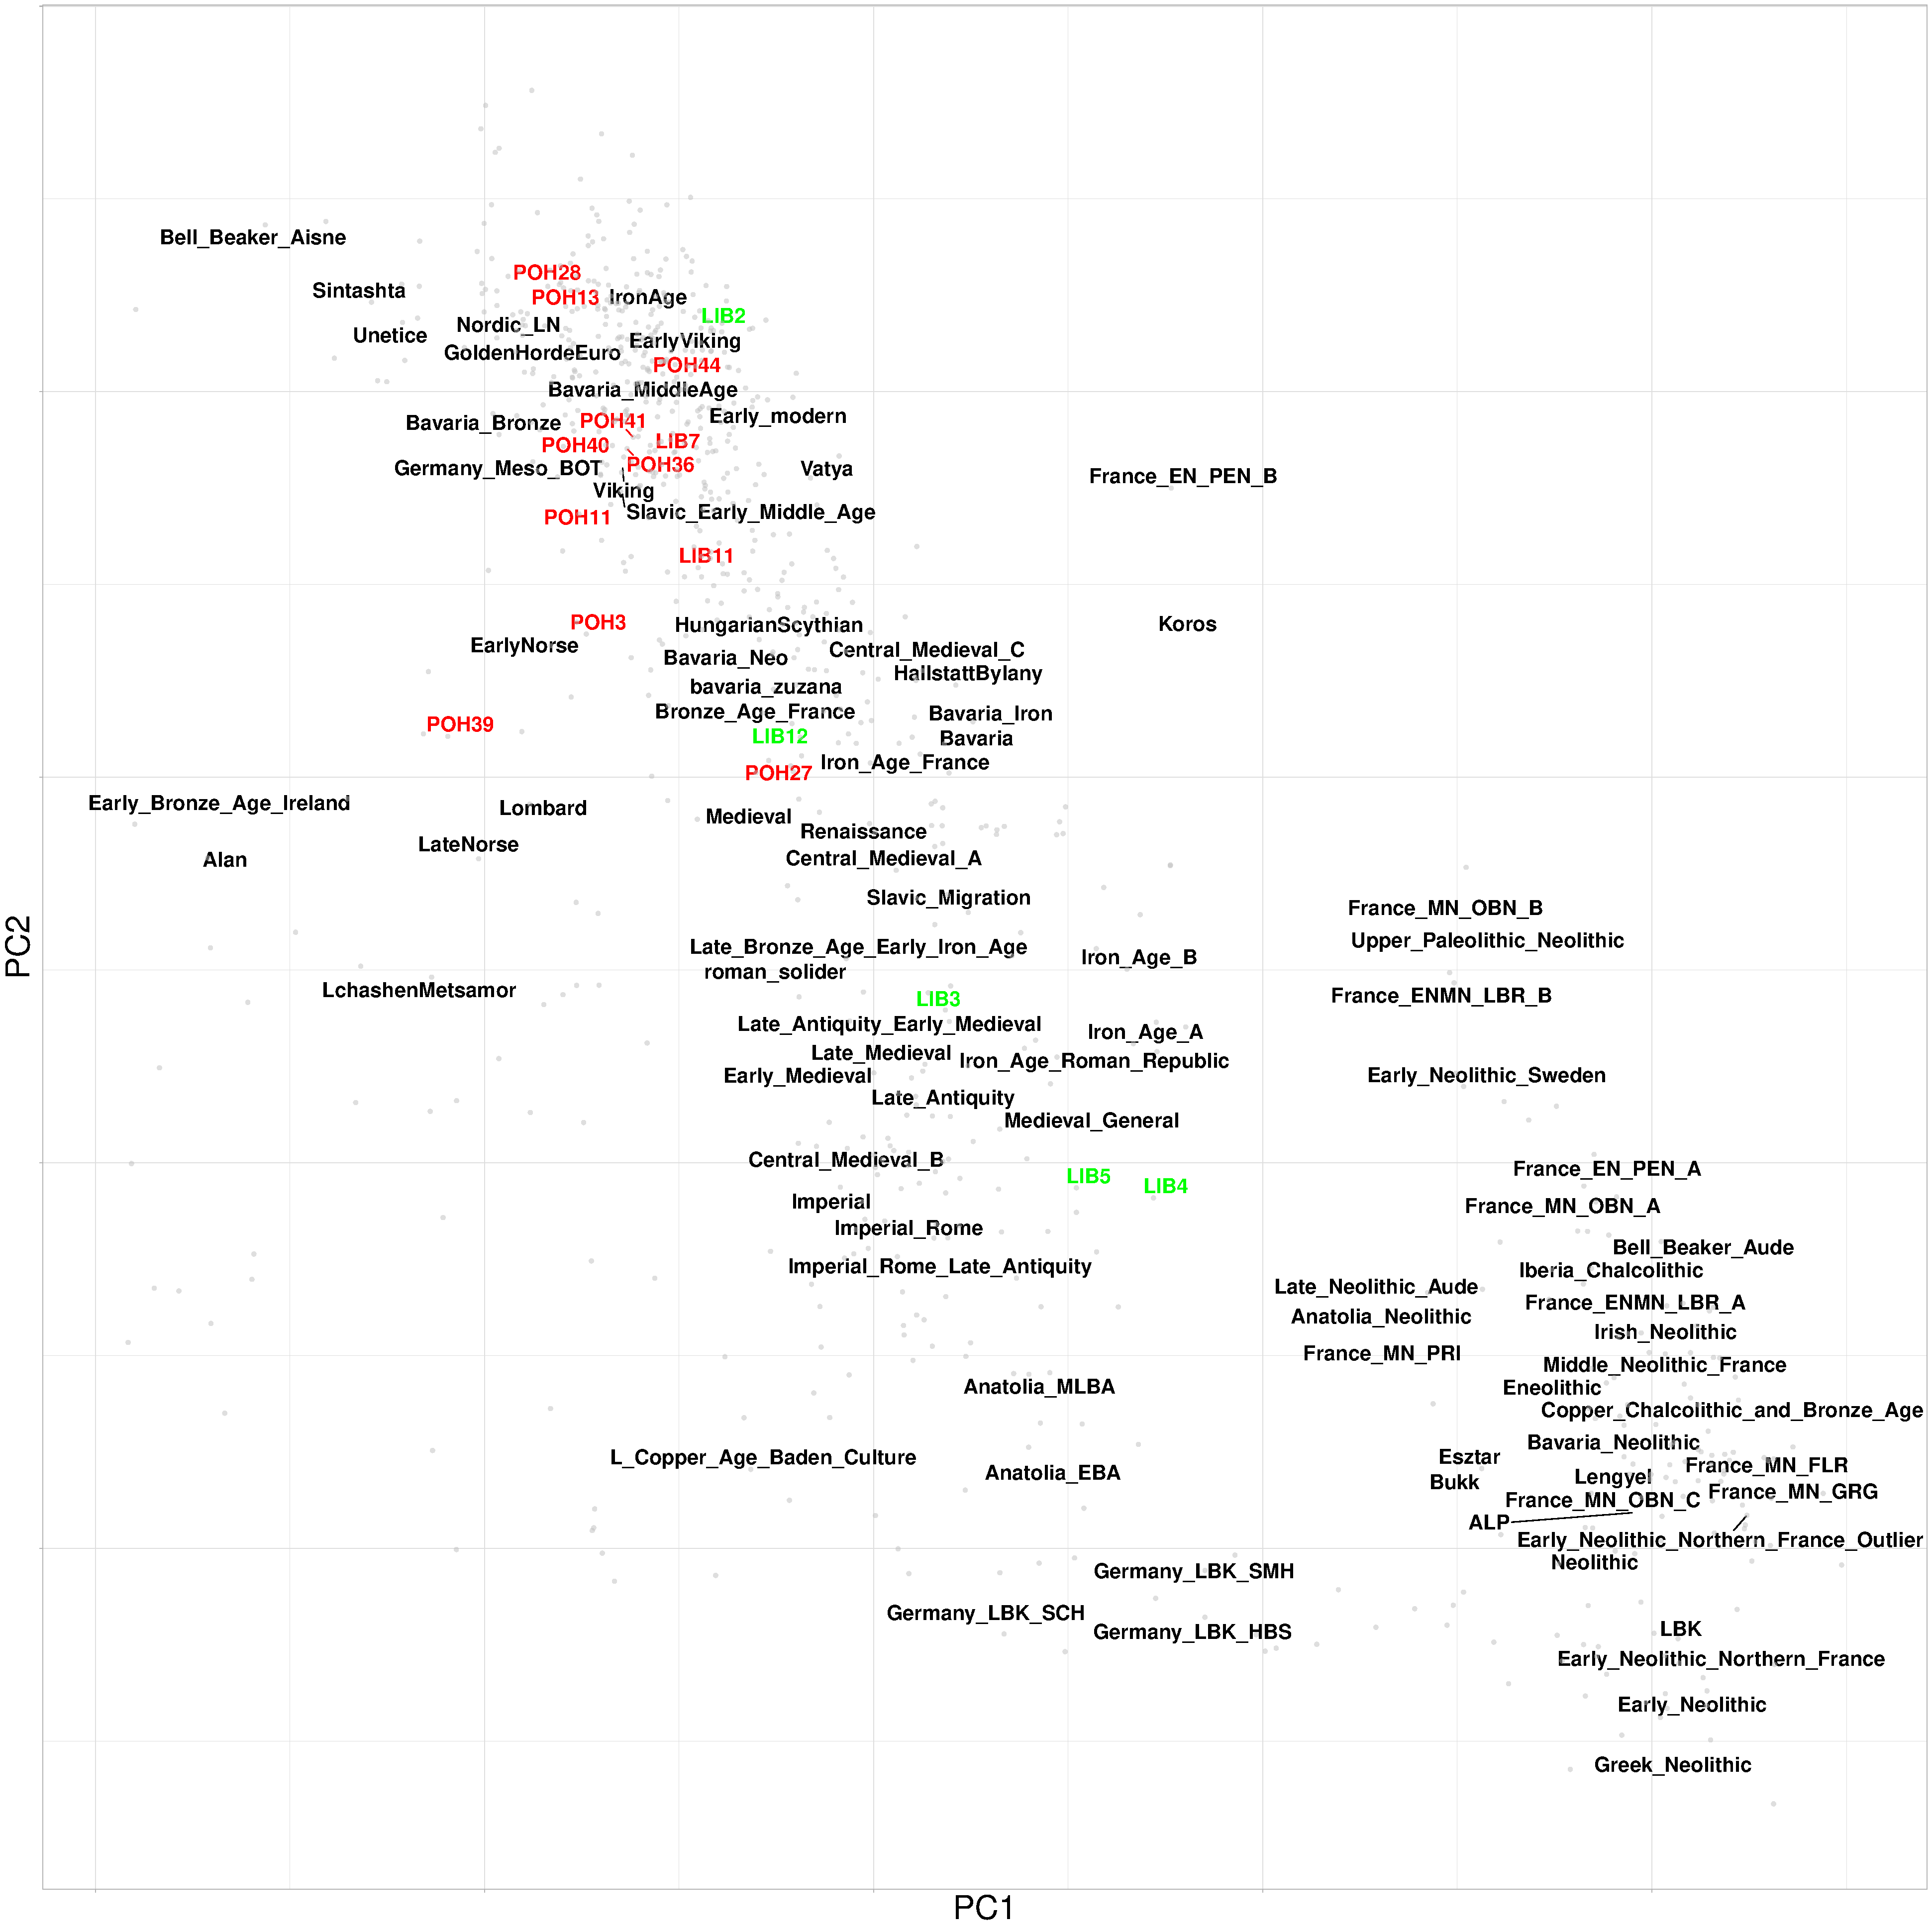
\includegraphics[width=1.0\textwidth]{../images/chapter5/plink_pca.pdf}
    \caption{Principle component plot of newly sequenced ancient samples and reference ancient individuals performed using the plink2. Green labels correspond to Migration Era samples, red labels to Early Middle Age samples and black as reference populations. The position of each reference label is the mean PC coordinates of all individuals within that population}
    \label{fig:AllChr.plink_PCA}
\end{figure}


\subsection{Mixed ancestry of Migration Period Slavs}

The Migration Period samples consisted of five individuals with radiocarbon dates corresponding to the Migration Period (348 - 509AD). Both the unlinked (Fig. \ref{fig:AllChr.plink_PCA}) and linked PCAs (Fig. \ref{fig:fs_PCA}) show that the Migration Period samples are heterogeneous and do not likely to originate from the same source population. One sample, LIB2 (495AD) is located in the centre of a large cluster of contemporaneous individuals from Iron Age central and northern Europe. fineSTRUCTURE grouped LIB2 with Viking era individuals from Sweden, Denmark, Iceland, Estonia and Norway from 300-1100AD. When painted using a set of present-day reference samples, LIB2 matches the most haplotypes and clusters with Norwegians (Fig. \ref{fig:copymatrix_moderns_ancient_slavs}). Put together, this data suggests LIB2 may be a recent migrant from Viking regions. 

\begin{figure}[htp]
    \centering
    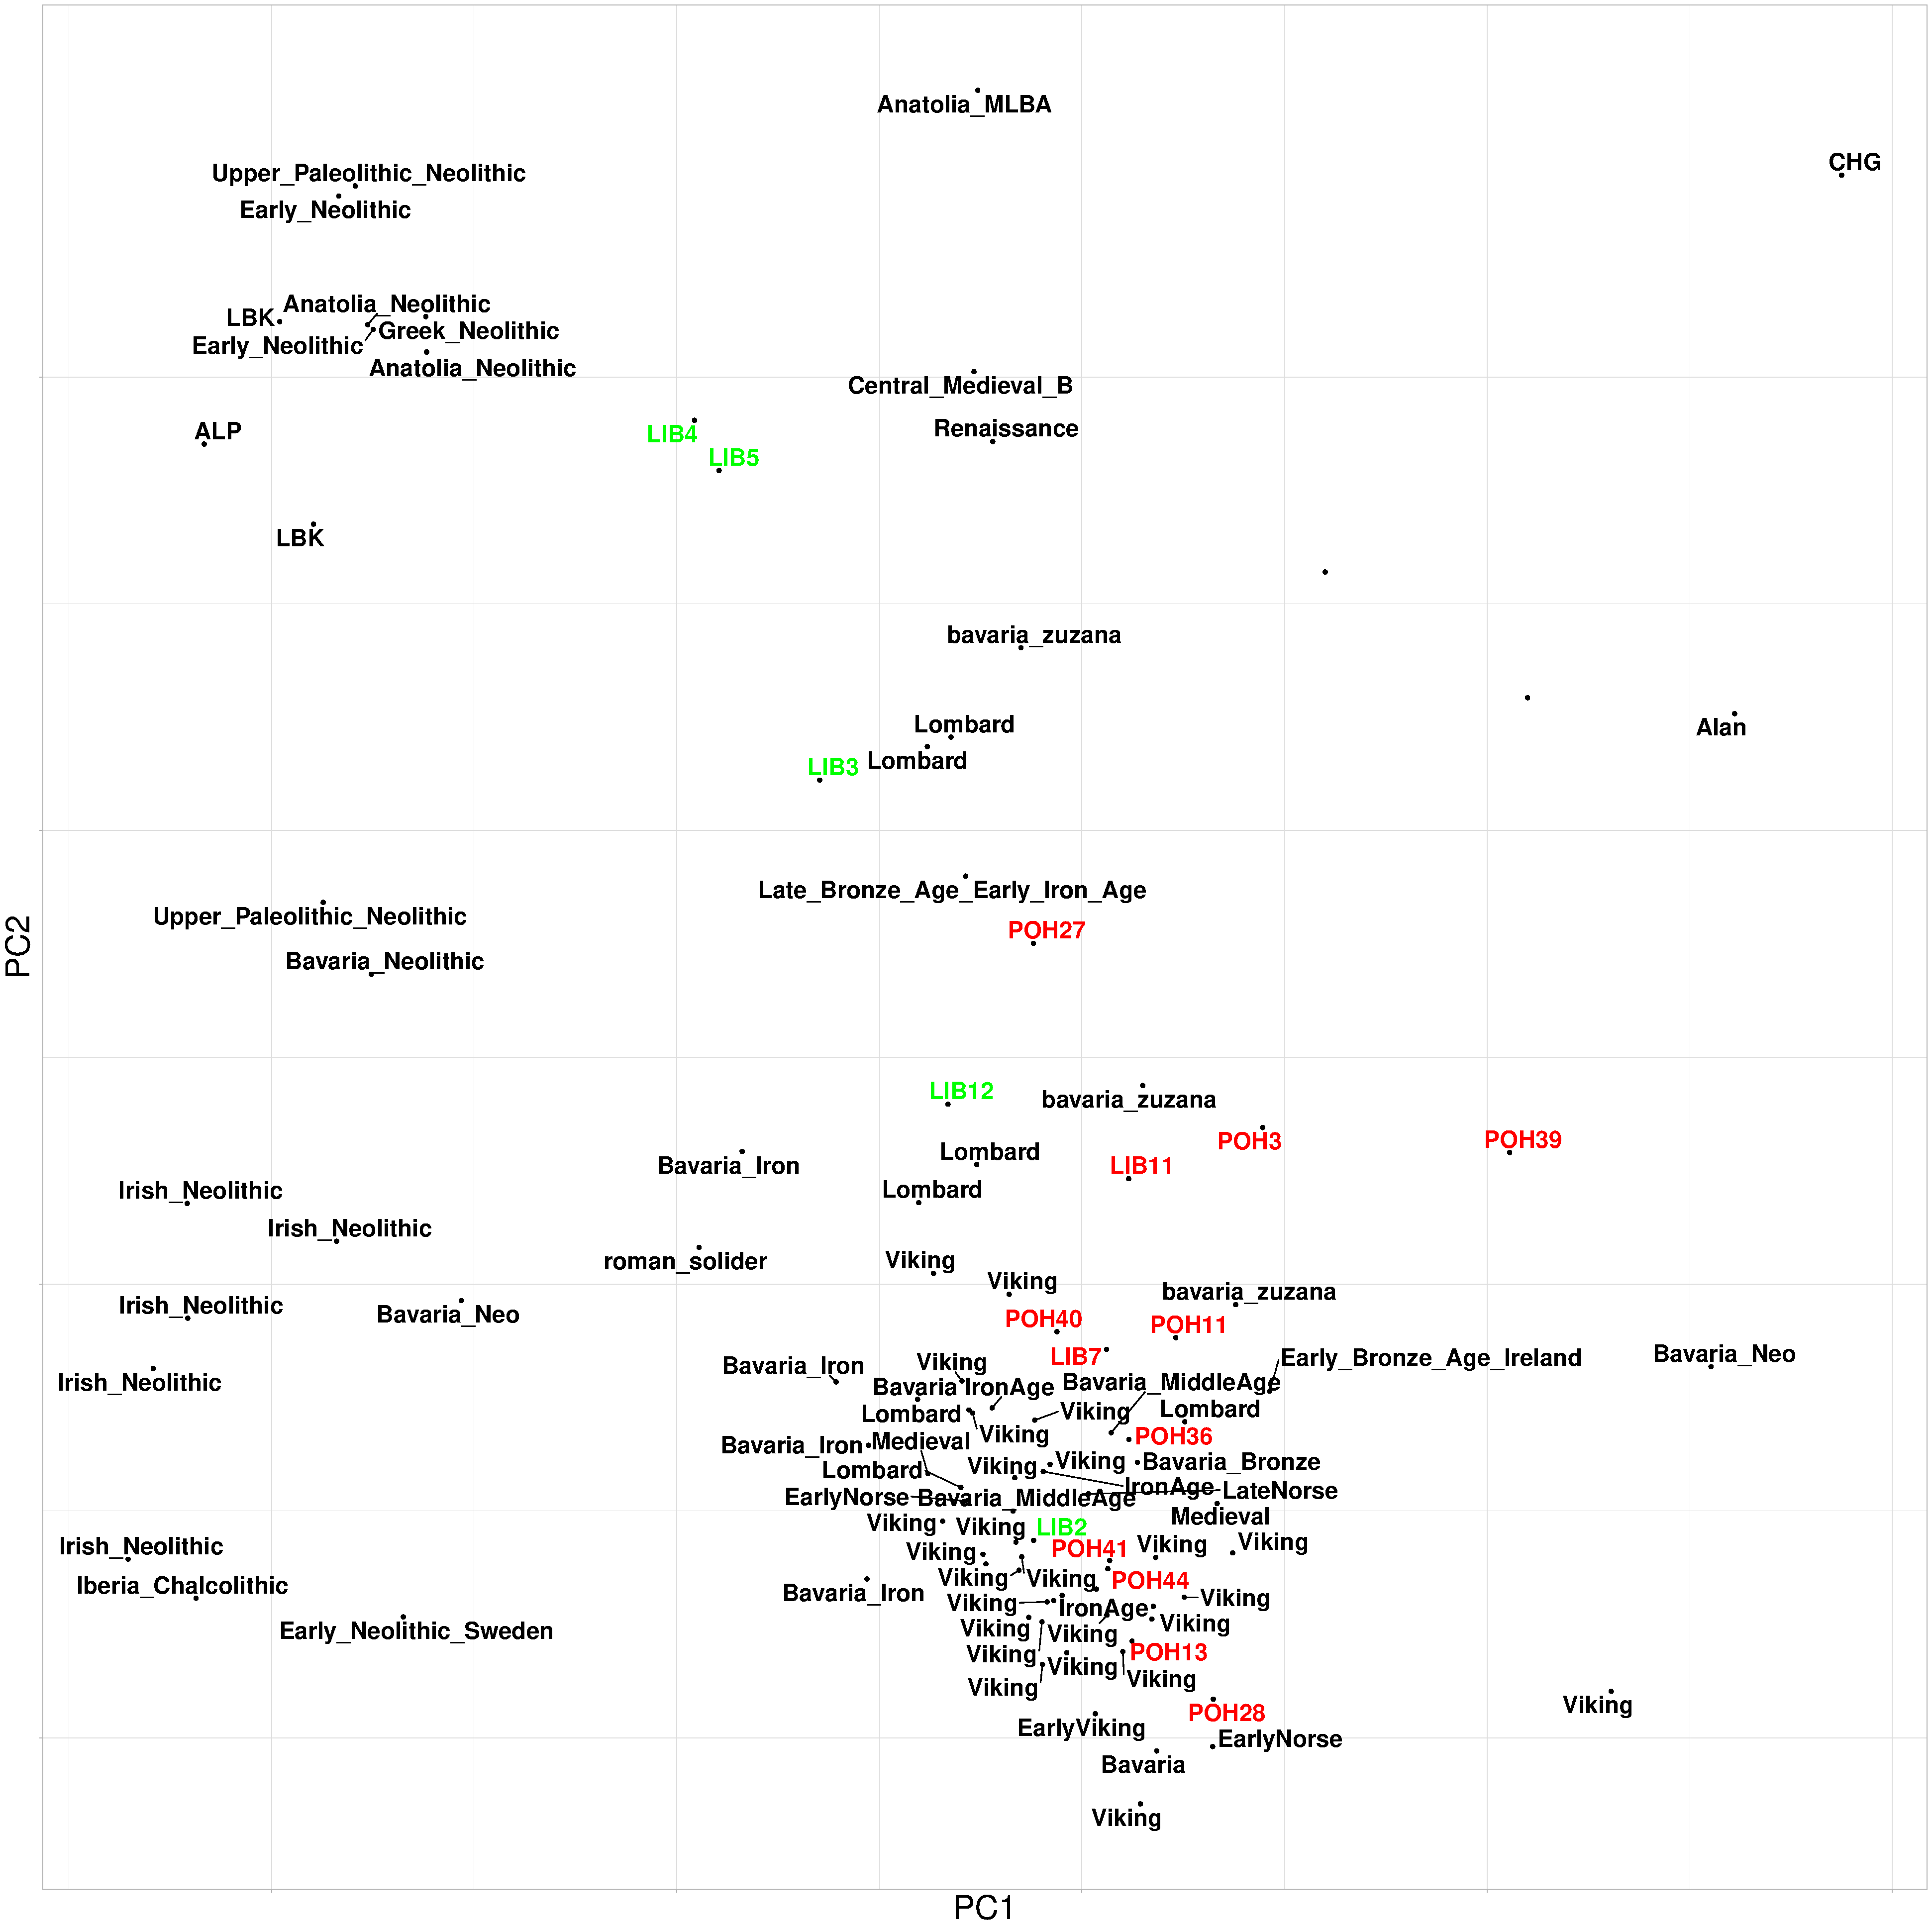
\includegraphics[width=1.0\textwidth]{../images/chapter5/fs_PCA.pdf}
    \caption{Principle component plot of newly sequenced ancient samples and reference ancient individuals performed using fineSTRUCTURE. Green labels correspond to Migration Era samples, red labels to Early Middle Age samples and black as reference populations.}
    \label{fig:fs_PCA}
\end{figure}

On the other hand, LIB4 and LIB5 are found in a fineSTRUCTURE group together with Early Iron Age and Renaissance samples from Italy, and generally show an increased affinity Neolithic / Southern European populations relative to the other Migration Period samples based on PCA results(Fig \ref{fig:AllChr.plink_PCA}-\ref{fig:fs_PCA}).

LIB3 clusters with Lombard samples from Northern Italy (Fig \ref{fig:AllChr.plink_PCA}) in the `ancient' painting, and with Tuscans in the `present-day' painting. Historical evidence cites alliances between Slavs and Lombards in the 5th century \cite{lotter2003volkerverschiebungen}. Finally, LIB12 displays ancestry which is more typical of the preceding Central European Bronze Age, suggesting it may represent a `leftover' from a local Bronze Age population which was unaffected by the Antiquity / Iron Age migrations to the region. It should be noted that the unlinked plink2 PCA and linked ChromoPainter PCA position LIB12 against slightly different other populations, with the unlinked PCA showing a similarity to Bronze and Iron Age French samples, and the linked PCA to Longobards and Bavarian samples. This may be caused by either the linked PCA giving higher resolution results, or giving details of a more ancient ancestral relationship.  

\subsection{Early Middle Age Slavs represent a relatively homogeneous group typical of European Middle Ages}

In comparison to the five Migration Period ancient Slavs, the 12 Early Middle Age Slavs (741-956 AD) are more homogeneous. All 12 samples cluster in the same fineSTRUCTURE group (named Slavic Early Middle Age II), alongside Viking/Medieval samples from Ukraine, Poland and Sweden. SOURCEFIND showed that the Slavic Early Middle Age II cluster derives roughly equal parts of ancestry from the clusters Viking 10C Scan I, BronzeAge I and Lombard mixed cluster. Interestingly, these three ancestry sources are similar to those identified by SOURCEFIND analyses in the Migration Period samples (Fig \ref{fig:SF_heatmap_slavs}). I tentatively therefore suggest that the Early Middle Age Slavs were formed from the mixture of `northern' (best represented by Viking) and `southern' ancestries (best represented by Lombards) onto a substrate of local Bronze Age populations.

MOSAIC admixture analysis on the Early Middle Age samples using ancient surrogates proved inconclusive. However, using present-day individuals as surrogates inferred a three-way admixture event involving sources closest to present-day day north-central Slavs (76.6\%), southern-eastern Slavs (21.9\%) and East Asians best represented by Mongolians (1.5\%) (Fig. \ref{fig:EarlyMiddleAges_MOSAIC_3way_moderns_Mu}). This admixture event was estimated to have occurred 9.4 (2.5\% 5.7gens - 97.5\% 17.9gens) generations before the samples (Fig. \ref{fig:EarlyMiddleAges_MOSAIC_3way_moderns_acoanc}), i.e.\ 476 - 732 AD. 

This admixture event is consistent with a signal inferred in both present-day day Eastern European individuals \cite{MOSAIC_2019, Hellenthal2014}. In previous studies, this admixture event was dated to approximately 1200CE (MOSAIC) and 440-1080 (GLOBETROTTER).

\begin{figure}[htp]
    \centering
    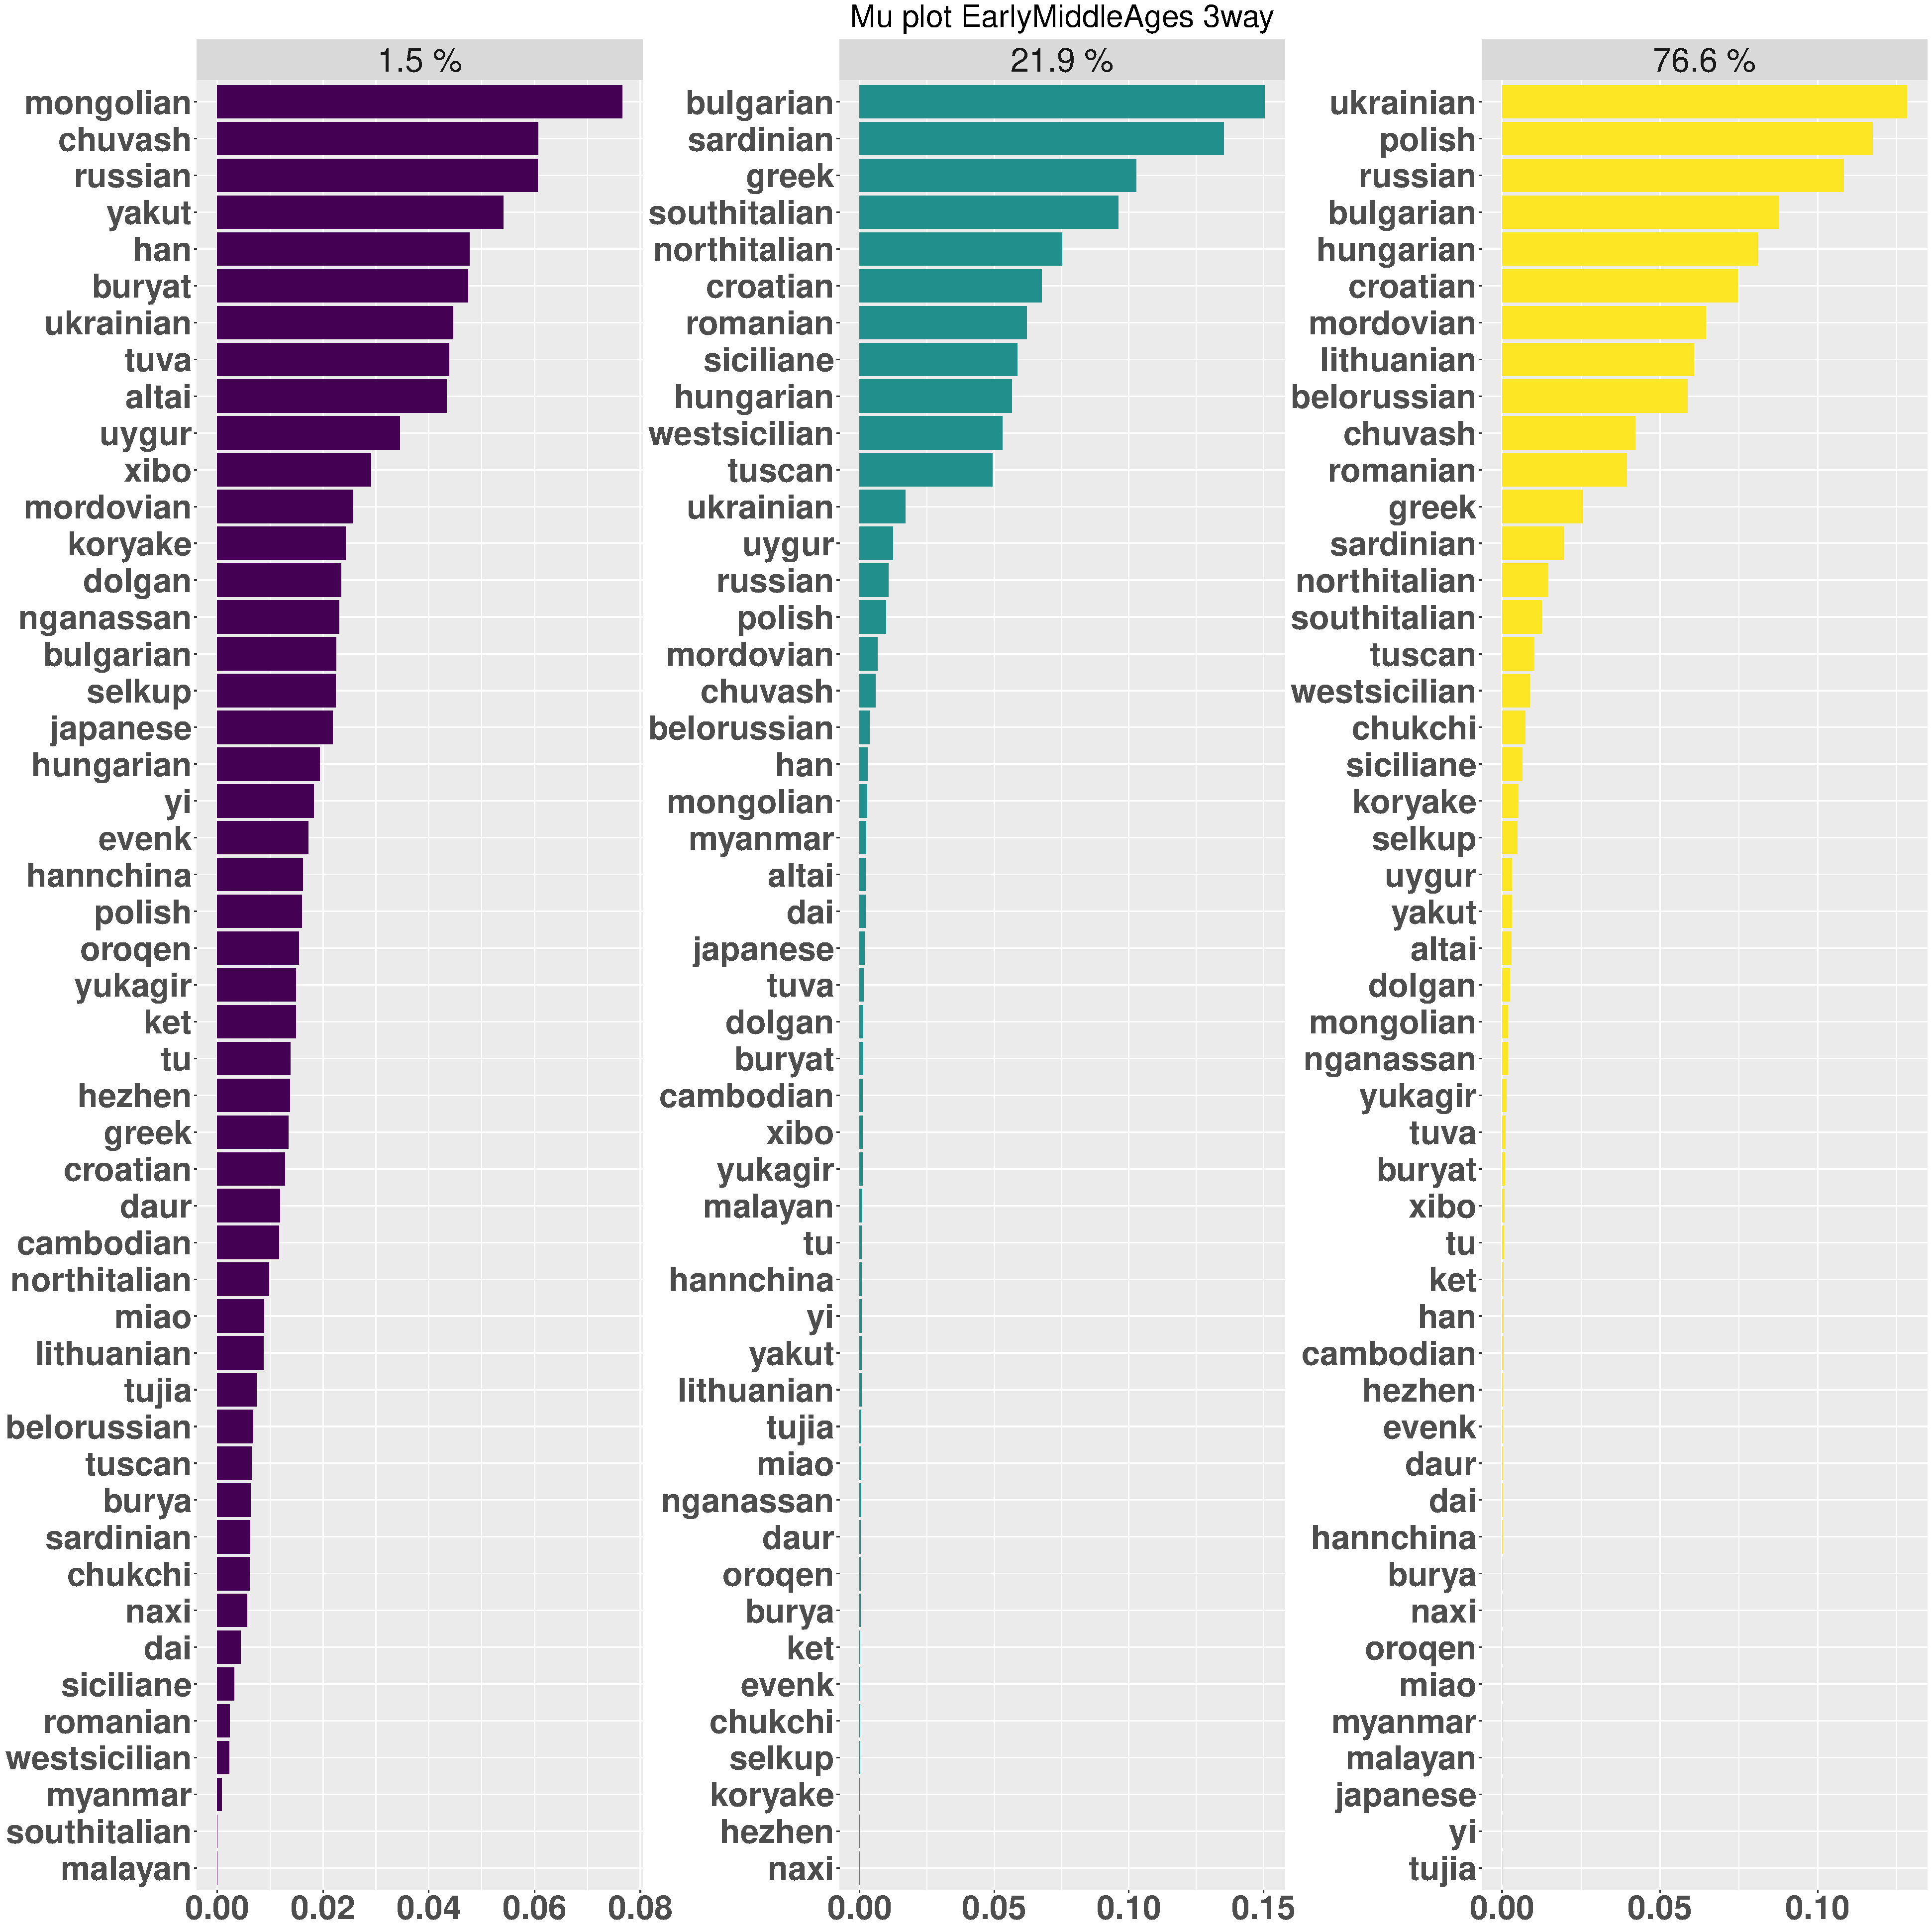
\includegraphics[width=1.0\textwidth]{../images/chapter5/Mu_plot_EarlyMiddleAges_3way.pdf}
    \caption{Copying matrix plot for sources in 3-way admixture event for Early Middle Age ancient Slavic samples. Each panel represents one of the 3 putative mixing sources. Labels above each panel gives the proportion that mixing source contributed to the Early Middle Age samples. Length of the bars within each panel represent the reflect how to best represent the relative haplotype composition of that source using the surrogate populations.}
    \label{fig:EarlyMiddleAges_MOSAIC_3way_moderns_Mu}
\end{figure}

\begin{figure}[htp]
    \centering
    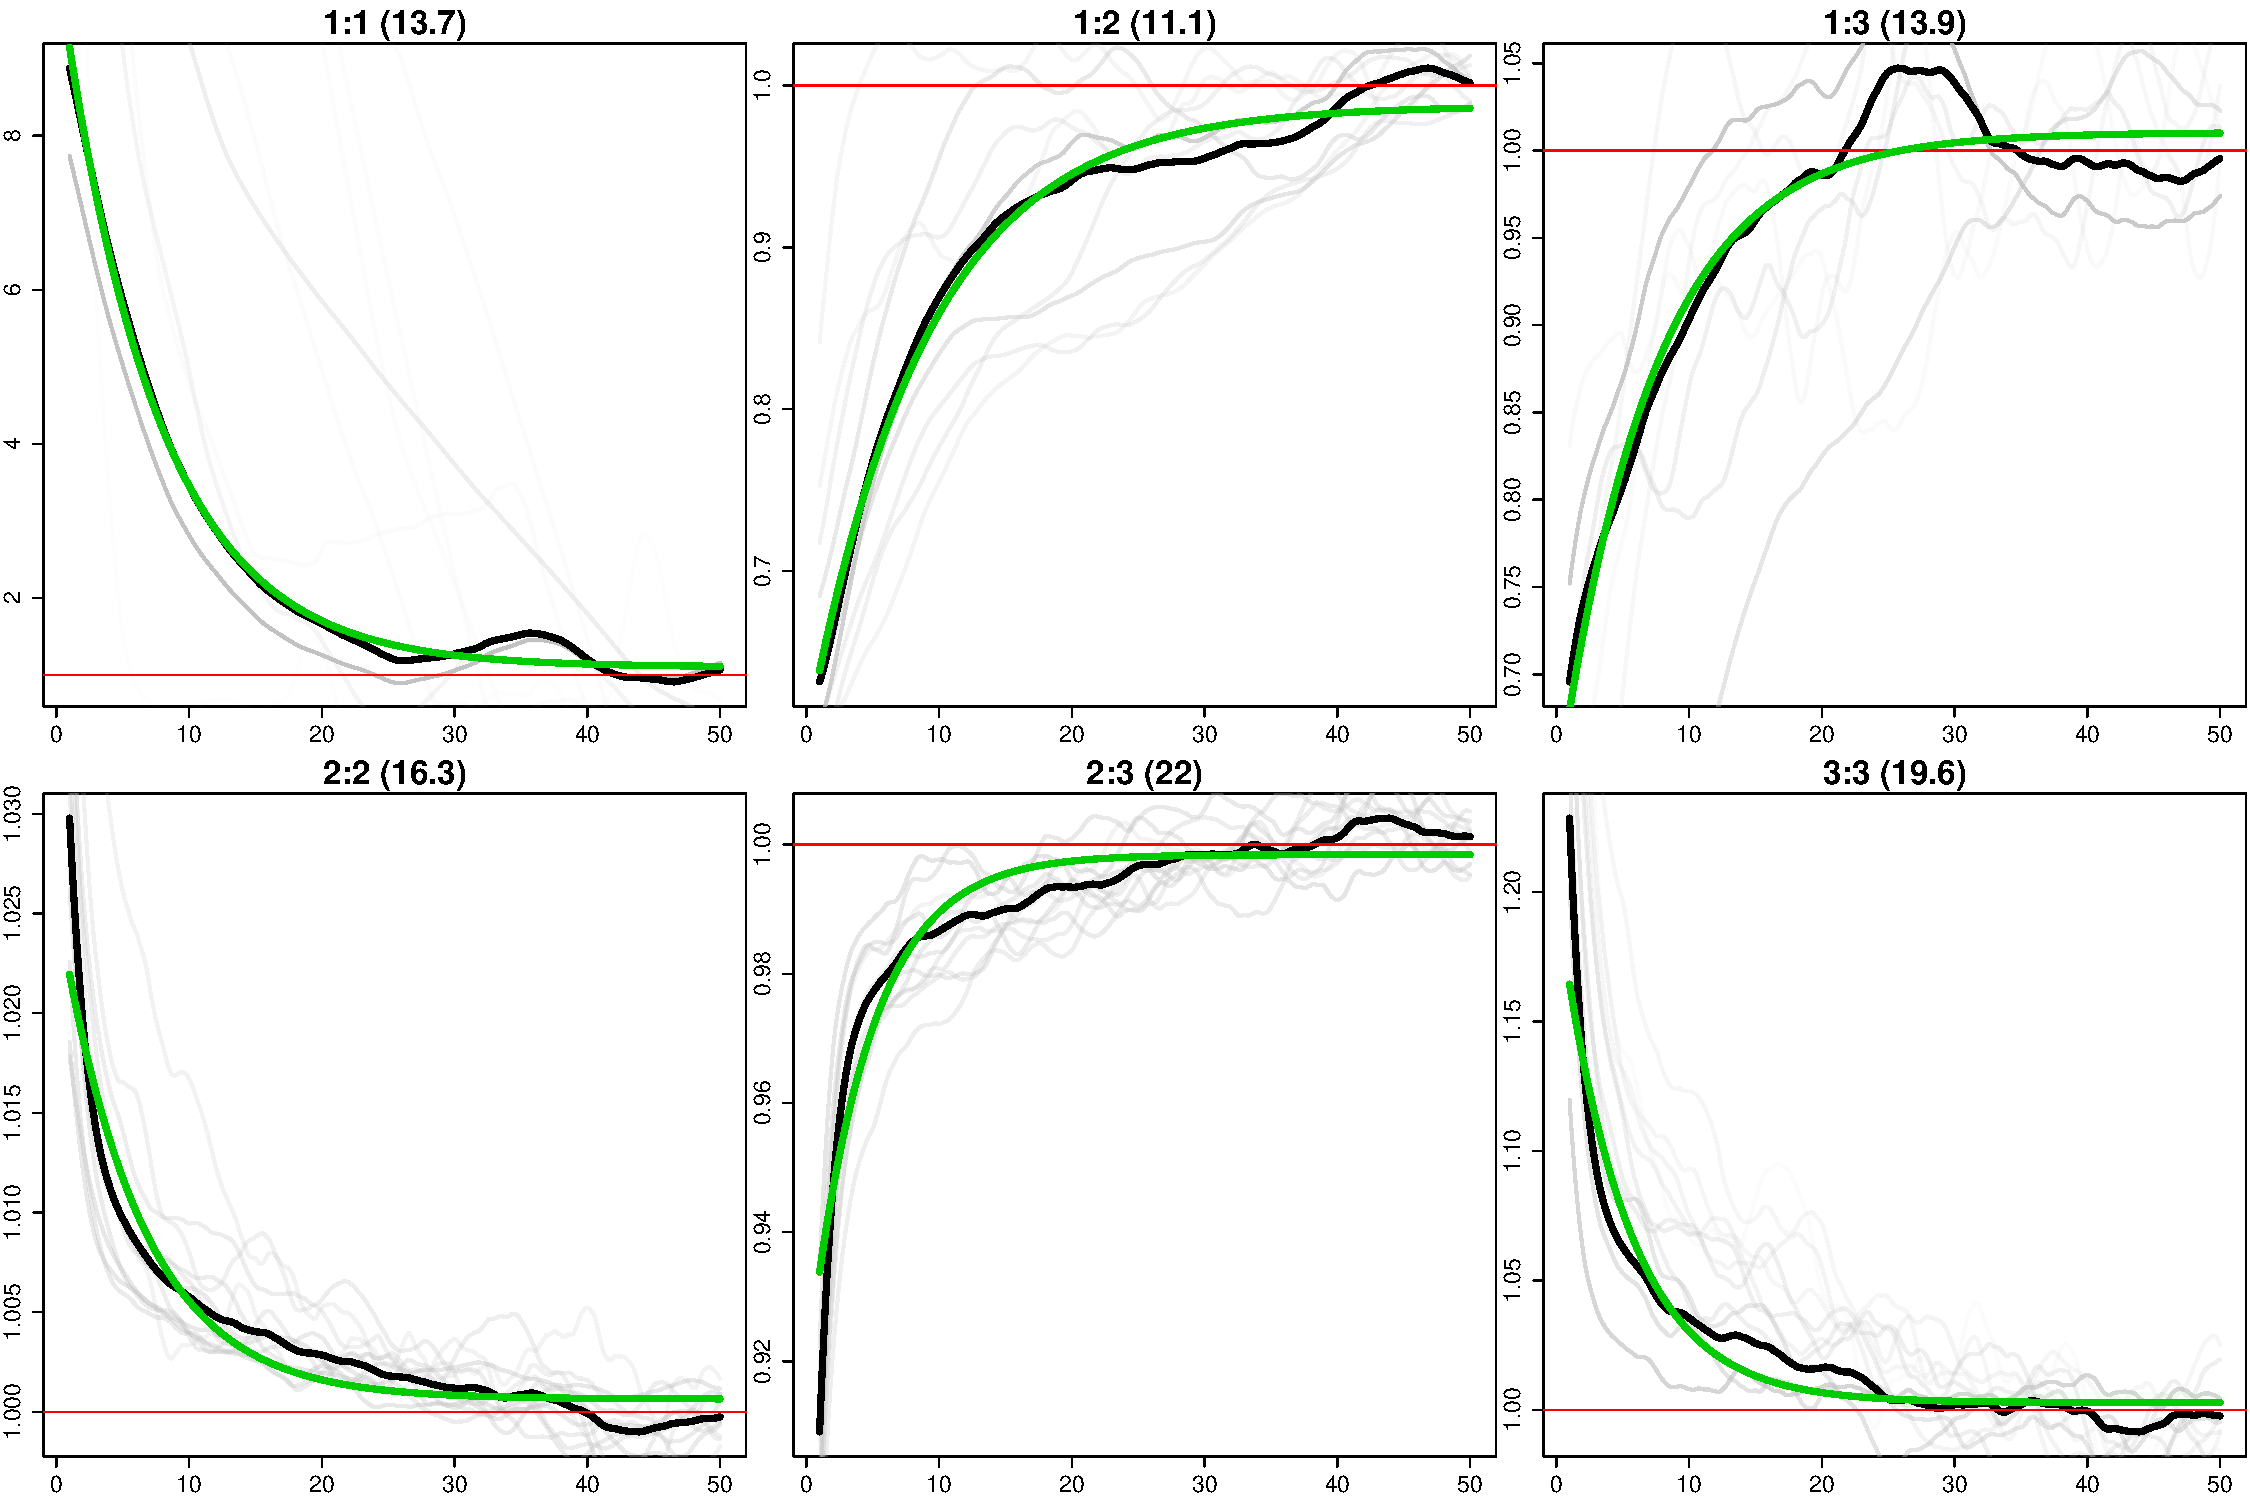
\includegraphics[width=1.0\textwidth]{../images/chapter5/EarlyMiddleAges_3way_acoanc.pdf}
    \caption{Inferred Coancestry Curves obtained from modelling Early Middle Age samples as a 3-way mixture of present-day individuals. Black lines are empirical coancestry curves across all target individuals, light grey are per individual, green is the fitted single-event coancestry curve. x-axis gives genetic distance and y-axis the probability of switching segments from source $a$ to source $b$. Sources are those given in Fig. \ref{fig:EarlyMiddleAges_MOSAIC_3way_moderns_Mu}.}
    \label{fig:EarlyMiddleAges_MOSAIC_3way_moderns_acoanc}
\end{figure}


\subsection{Assessing continuity between Early Middle Age and Migration Period samples} \label{sec:TVD_test}

To formally establish whether the Early Middle Age and Migration Period samples cluster within their respective populations to the exclusion of the other, following Leslie et al 2015 \cite{Leslie2015}, I performed a TVD permutation test. Full details of $TVD$ justification and calculation are outlined in Appendix section \ref{sec:appendixTVD}.

Using the ancients chunklengths matrix, I grouped the samples into Migration Period and Early Middle Age and calculated the average copyvectors $C_{mp}$ and $C_{ema}$ across samples within each groups. Here $C_{mp}=\{C_{mp}(1),...,C_{mp}{D}\}$, where $C_{mp}(d)$ is the average amount a Migration Period individual copies from (i.e.\ is painted by) individuals from donor population $d$. Then, I calculated the empirical TVD between the two groups as $TVD_{mp,ema} = \sum_d |C_{mp}(d) - C_{ema}(d)|$. For 10,000 iterations, I then randomly permuted the population labels among the samples and then calculated the analogous TVD, $TVD_{mp,ema}^{rand}$, between these two randomised ``populations''. I then calculated, as a p-value for the null model assuming individuals are exchangeable between the two populations, the number of randomly permuted iterations where $TVD_{mp,ema}^{rand} \geq $ $TVD_{mp,ema}$. This test supported clustering the samples into their respective groups ($p=0.0013$).

To determine the extent of continuity between the Migration Period and Early Middle Ages, I modelled each Early Middle Ages sample as a mixture of other ancients, including individuals from the preceding Migration Period, using SOURCEFIND. The proportion of ancestry derived from the Migration Period was low (mean 3.4\% , range 0.4\% - 12.5\%), suggesting that there was a relatively large scale population replacement between the two different time periods. 

\subsection{Legacy of Slavic migrations in present-day individuals}

Principle component analysis (PCA) of the present-day painting indicates genetic similarity between ancient Slavic samples from the Early Middle Ages and present-day day Slavic speaking populations (Fig. \ref{fig:chunklengths_moderns_ancients_PCA}). The Early Middle Age samples primarily cluster with present-day Polish and Belorussian individuals, but appear to fall on a cline of genetic similarity between Russians and southern Europeans. 

As with the ancients PCA, Migration Era Slavs are spread across the present-day PCA. LIB3, LIB4, and LIB5 cluster with present-day Italians, consistent with deriving a substantial ancestry component from southern European sources. LIB4 and LIB5 appear to be positioned closer to southern Italians and Greeks, whereas LIB3 is closer to northern Italian and Tuscan populations. LIB2 shows a strong affinity to present-day Norwegians, suggesting it may be a recent migrant from Viking regions. 

\begin{figure}[htp]
    \centering
    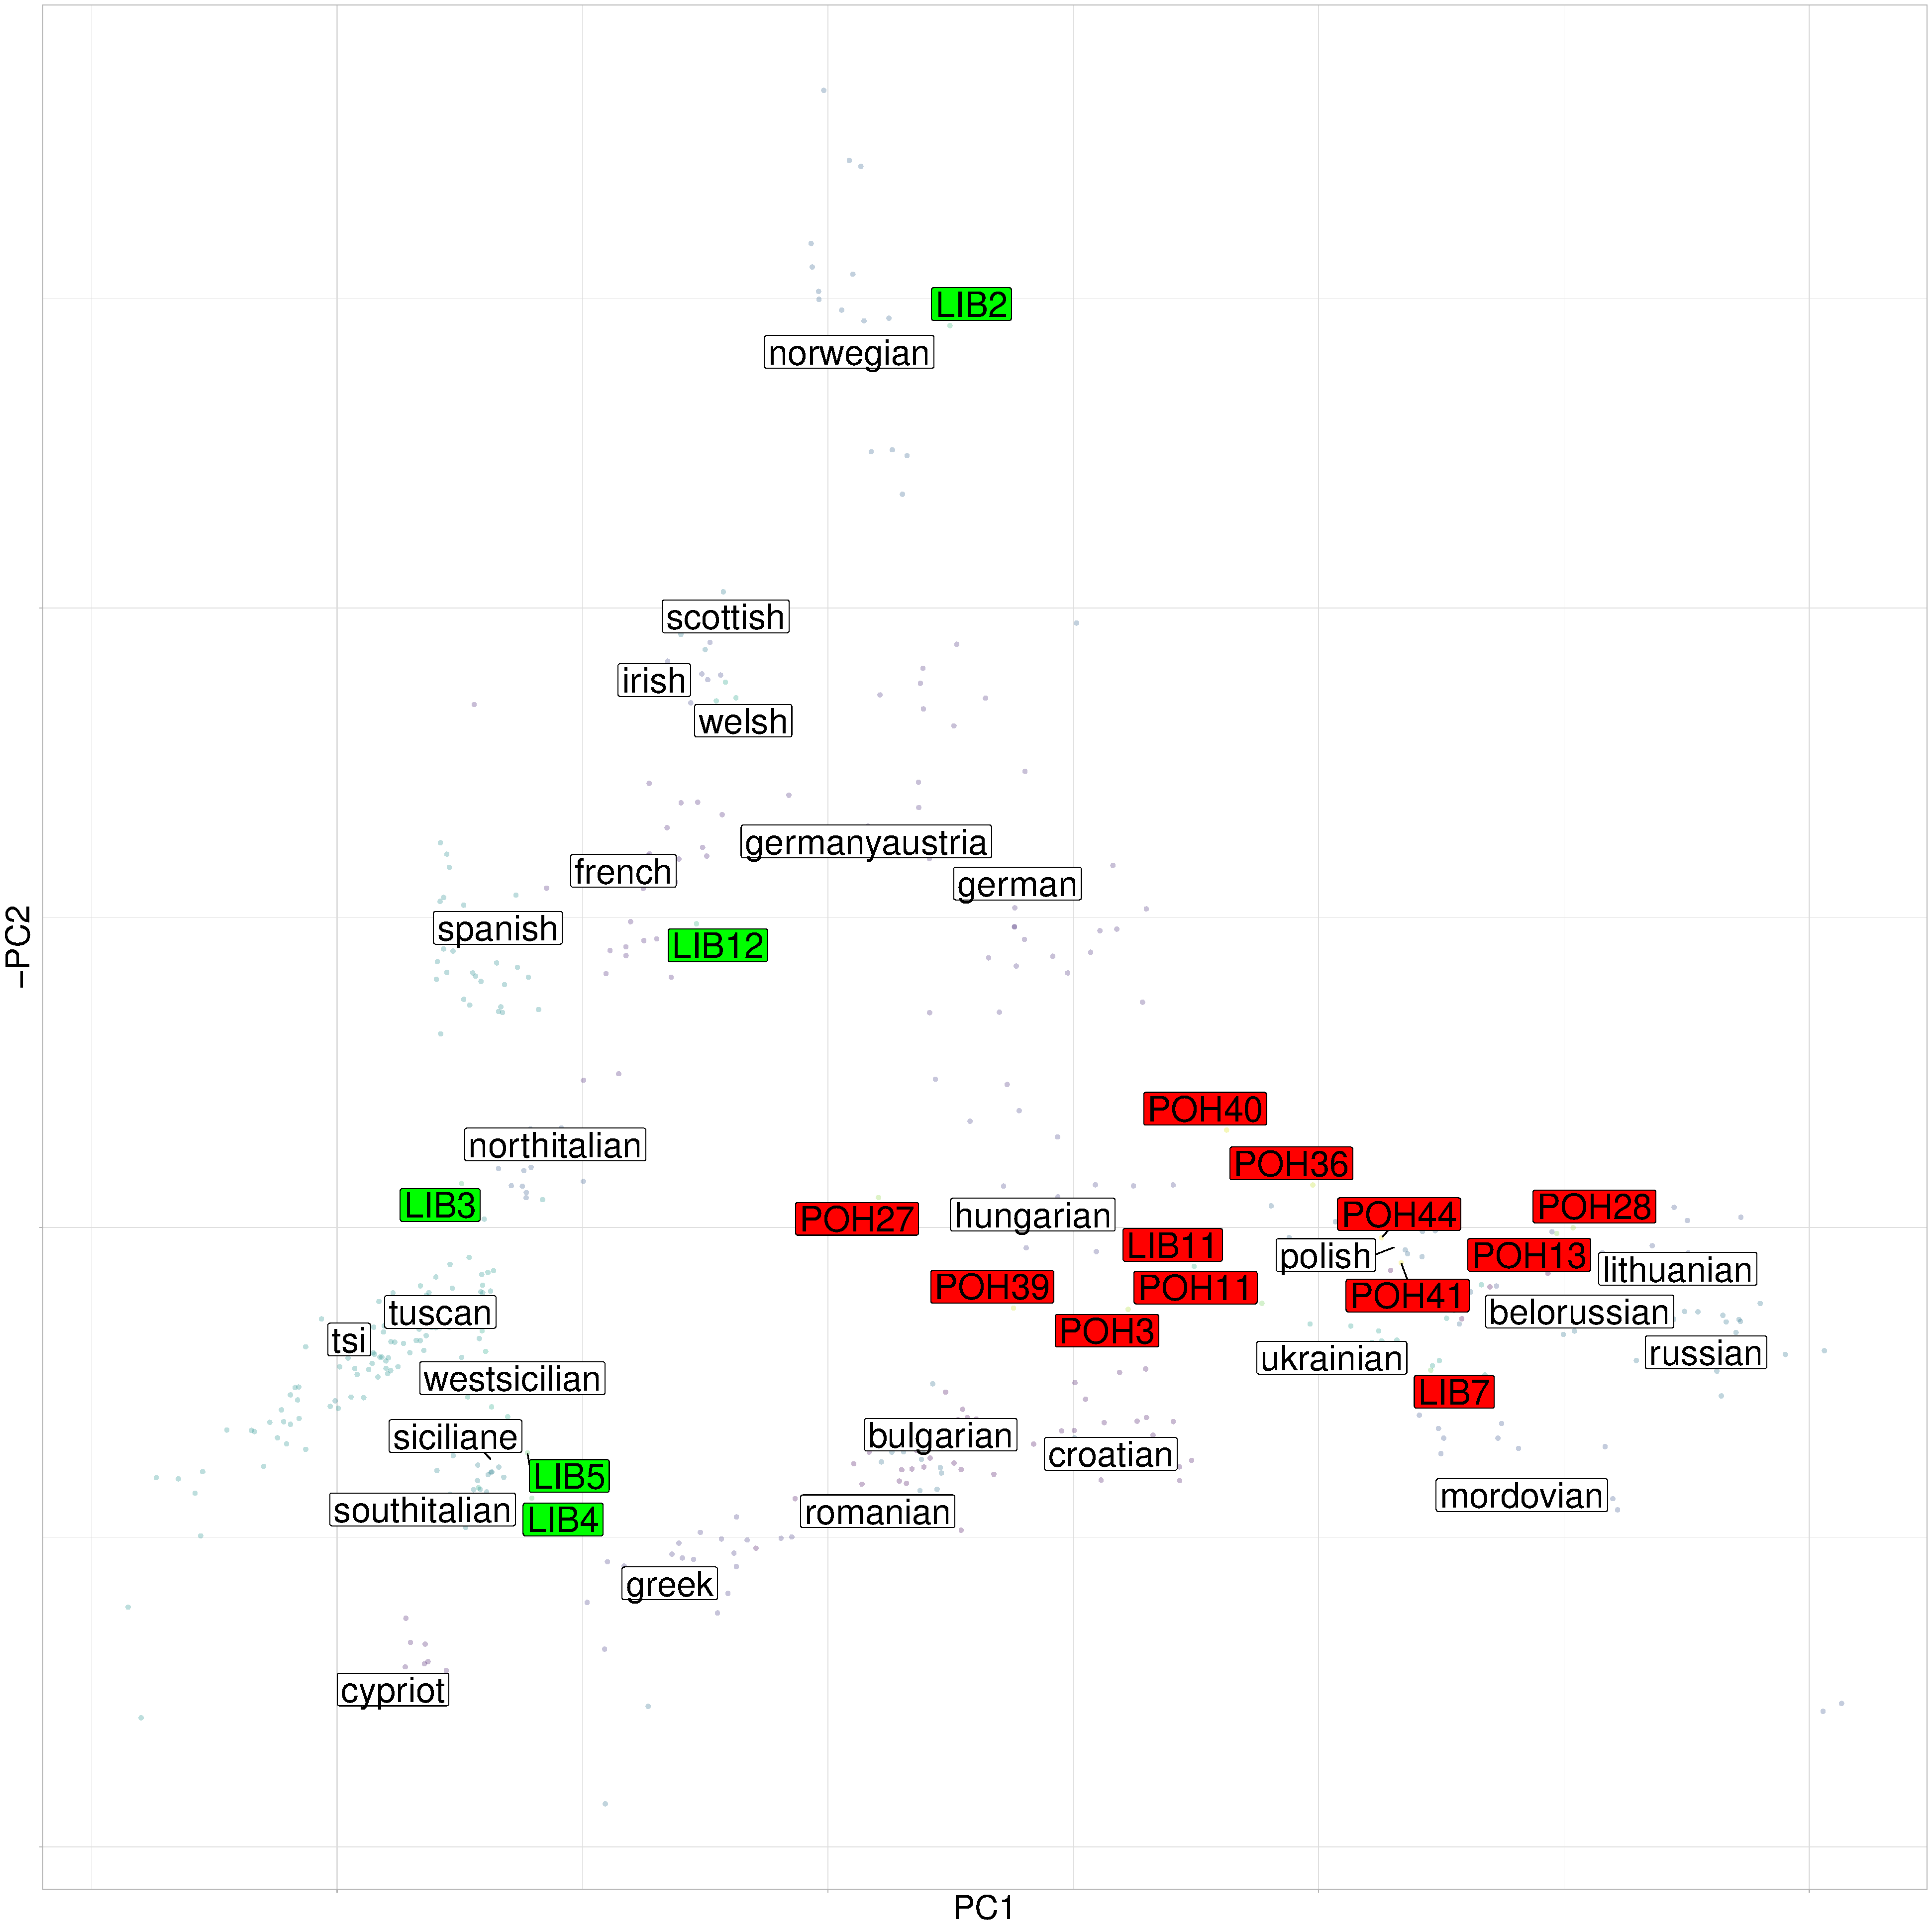
\includegraphics[width=1.0\textwidth]{../images/chapter5/chunklengths_moderns_ancients_PCA.pdf}
    \caption{Principle component plot of newly sequenced ancient samples and reference modern individuals performed using the finestructure library. Green labels correspond to Migration Era samples, red labels correspond to Early Middle Age samples and white labels correspond to reference populations. The position of each reference label is the mean PC coordinates of all individuals within that population. Transparent coloured points correspond to present-day individuals.}
    \label{fig:chunklengths_moderns_ancients_PCA}
\end{figure}

The same pattern can be observed on the raw copyvector output matrix from the present-day painting (Fig. \ref{fig:copymatrix_moderns_ancient_slavs}). In particular, Migration Era samples show little excess affinity to present-day day Slavic populations and more affinity to present-day Greek individuals. 

\begin{figure}[htp]
    \centering
    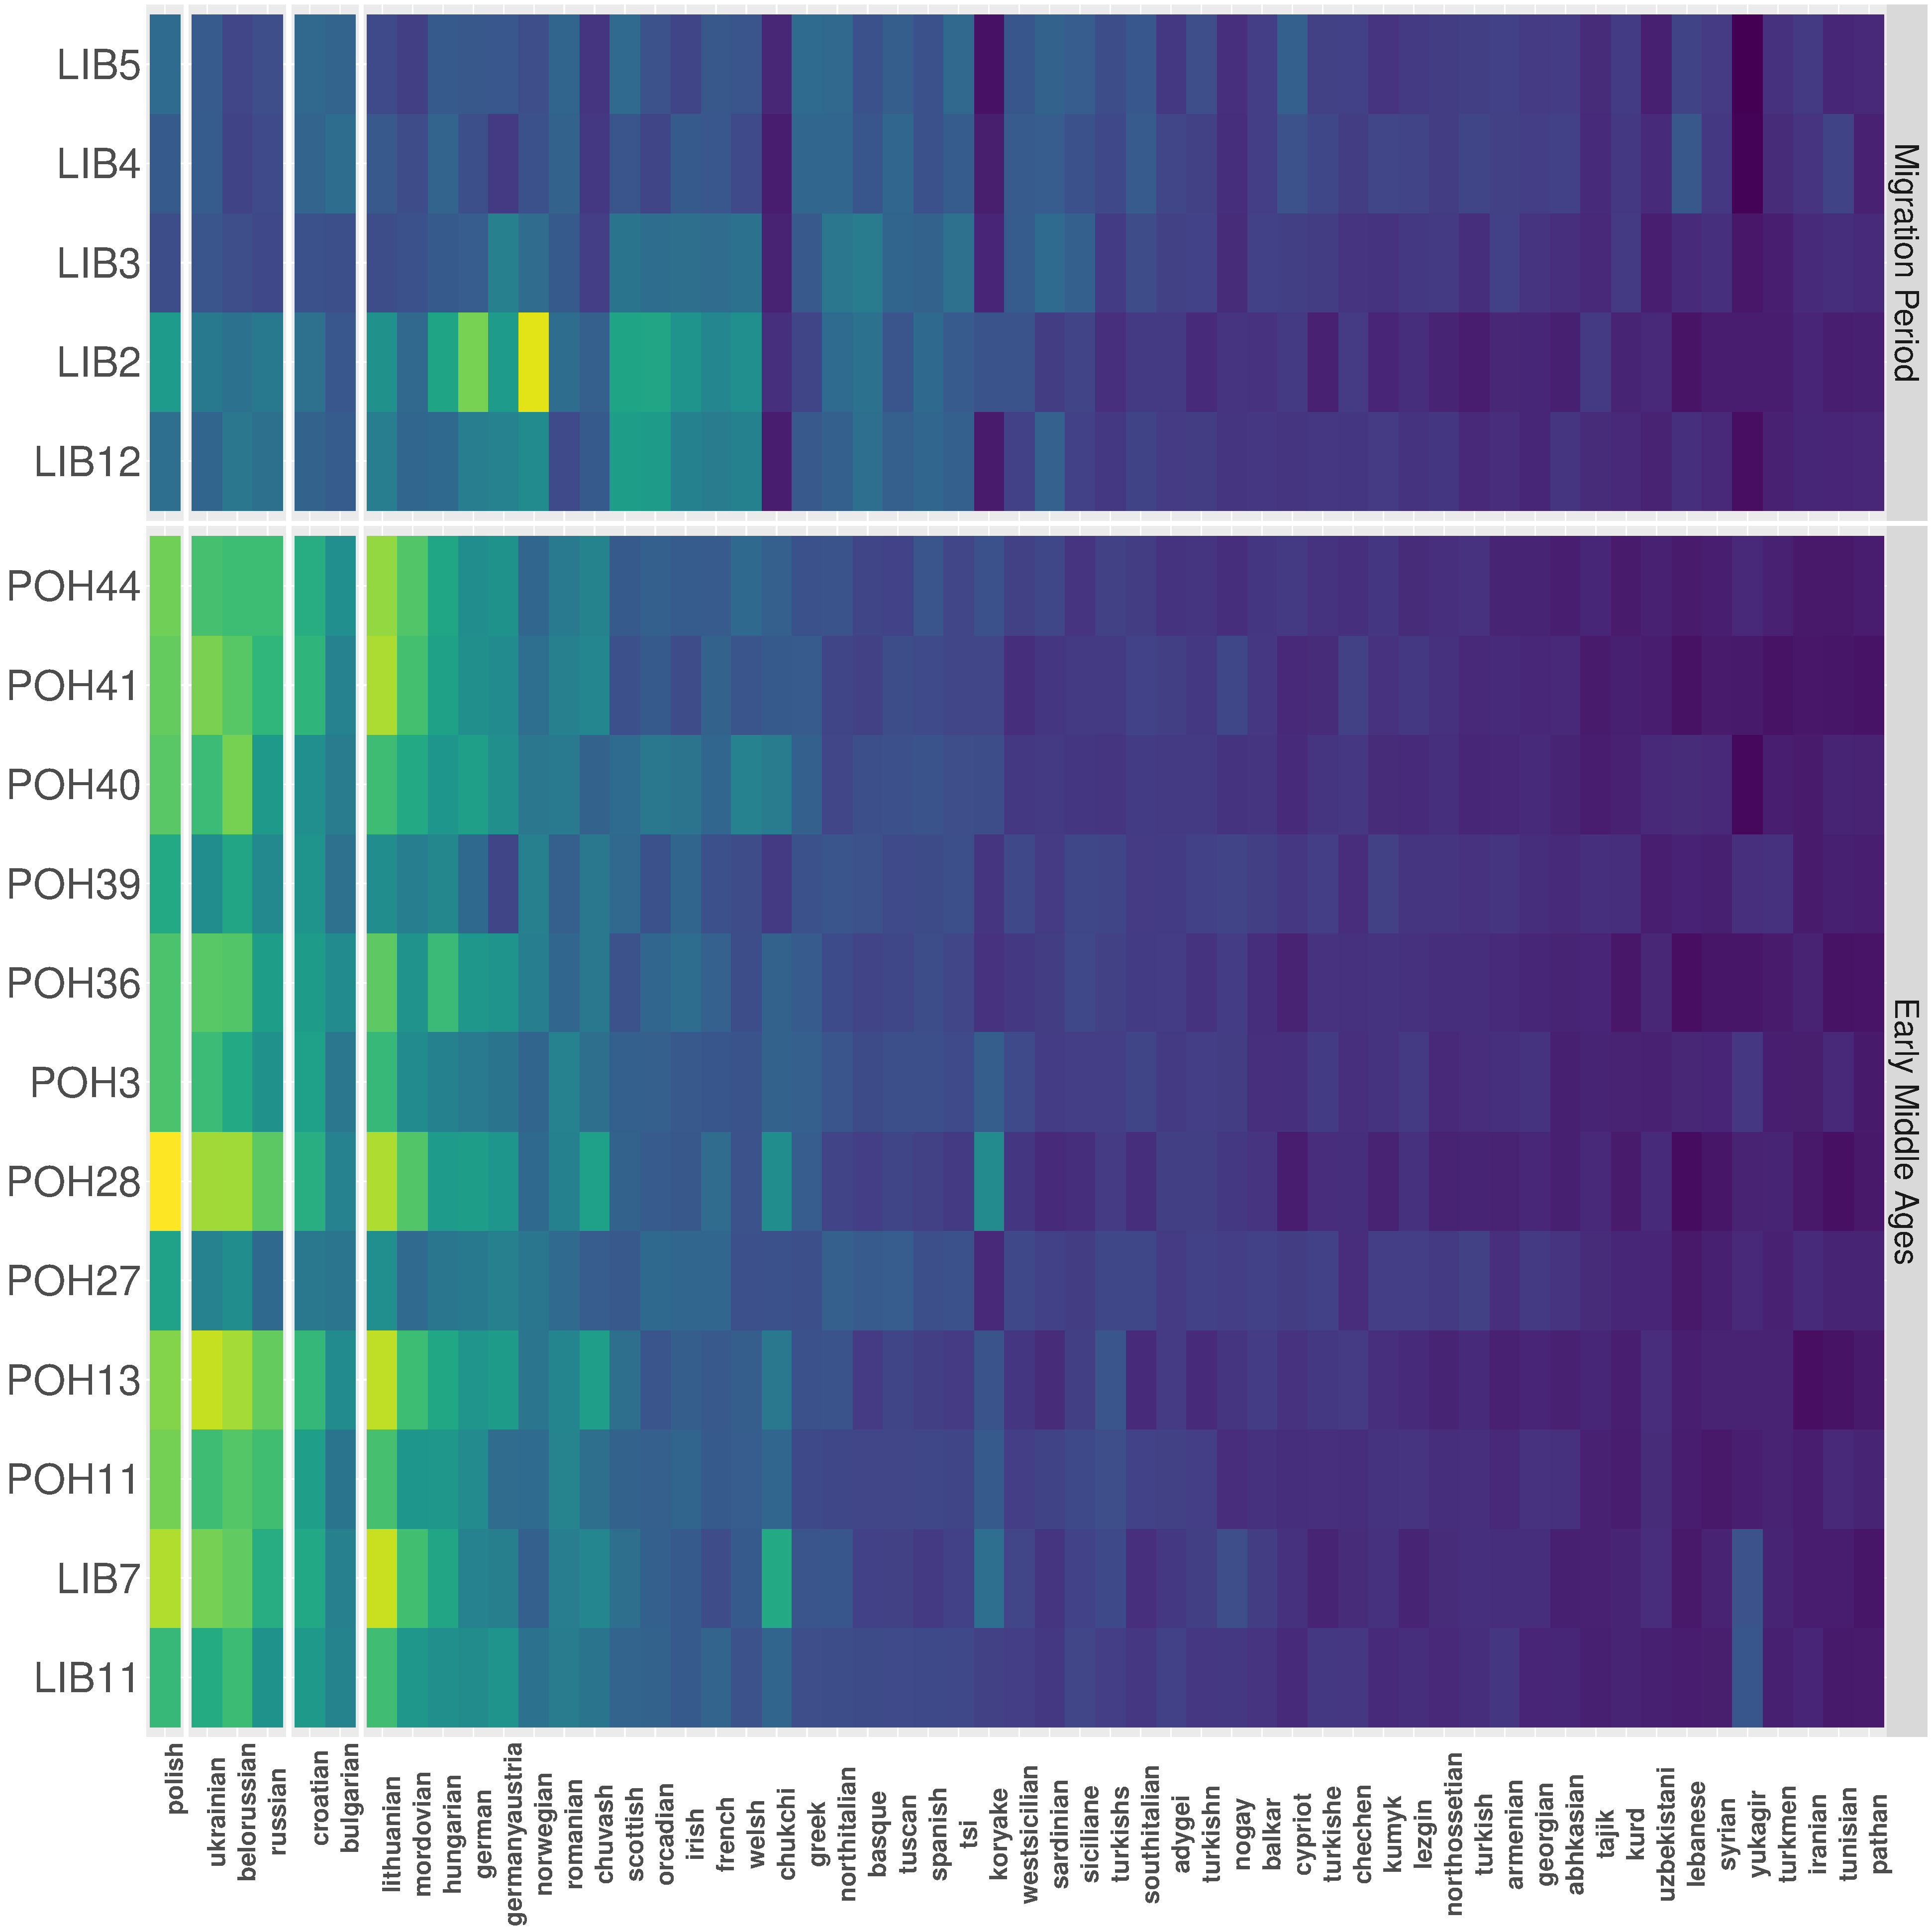
\includegraphics[width=1.0\textwidth]{../images/chapter5/copymatrix_moderns_ancient_slavs.pdf}
    \caption{Raw chunklengths matrix from the `present-day' painting. Rows correspond to different ancient recipient individuals, grouped into Migration Period and Early Middle Age period, and columns to different donor populations. Colour of cells corresponds to the total length of genome that a given donor individuals donates to that recipient, with dark/blue  indicating less sharing and light/yellow colours indicating more sharing.}
    \label{fig:copymatrix_moderns_ancient_slavs}
\end{figure} 

In contrast, the Early Middle Age samples showed a strong affinity to present-day day Slavic populations, especially Polish, Lithuanians and Mordovians. 

To confirm that the observed results were not a result of phasing or imputing ancient individuals using present-day samples, I calculated $f_{3}$ statistics on pre-imputation genotypes. Specifically, I calculated $f_{3}$, or the branch length / amount of shared drift, between a set of present-day test populations and the grouped Early Middle Age samples. The results are qualitatively similar to those obtained using ChromoPainter, with Early Middle Age ancient Slavic individuals being closest to samples from Eastern Europe (Fig. \ref{fig:f3_HB_ancient_slavs}). However, the $f_{3}$ results do not appear to show the same degree of geographical structure; for example, Early Middle Age have a more positive $f_{3}$ with present-day Irish individuals than with some present-day Slavic-speaking groups such as Croatians, perhaps reflecting relatively higher genetic drift in the Irish population.

\begin{figure}[htp]
    \centering
    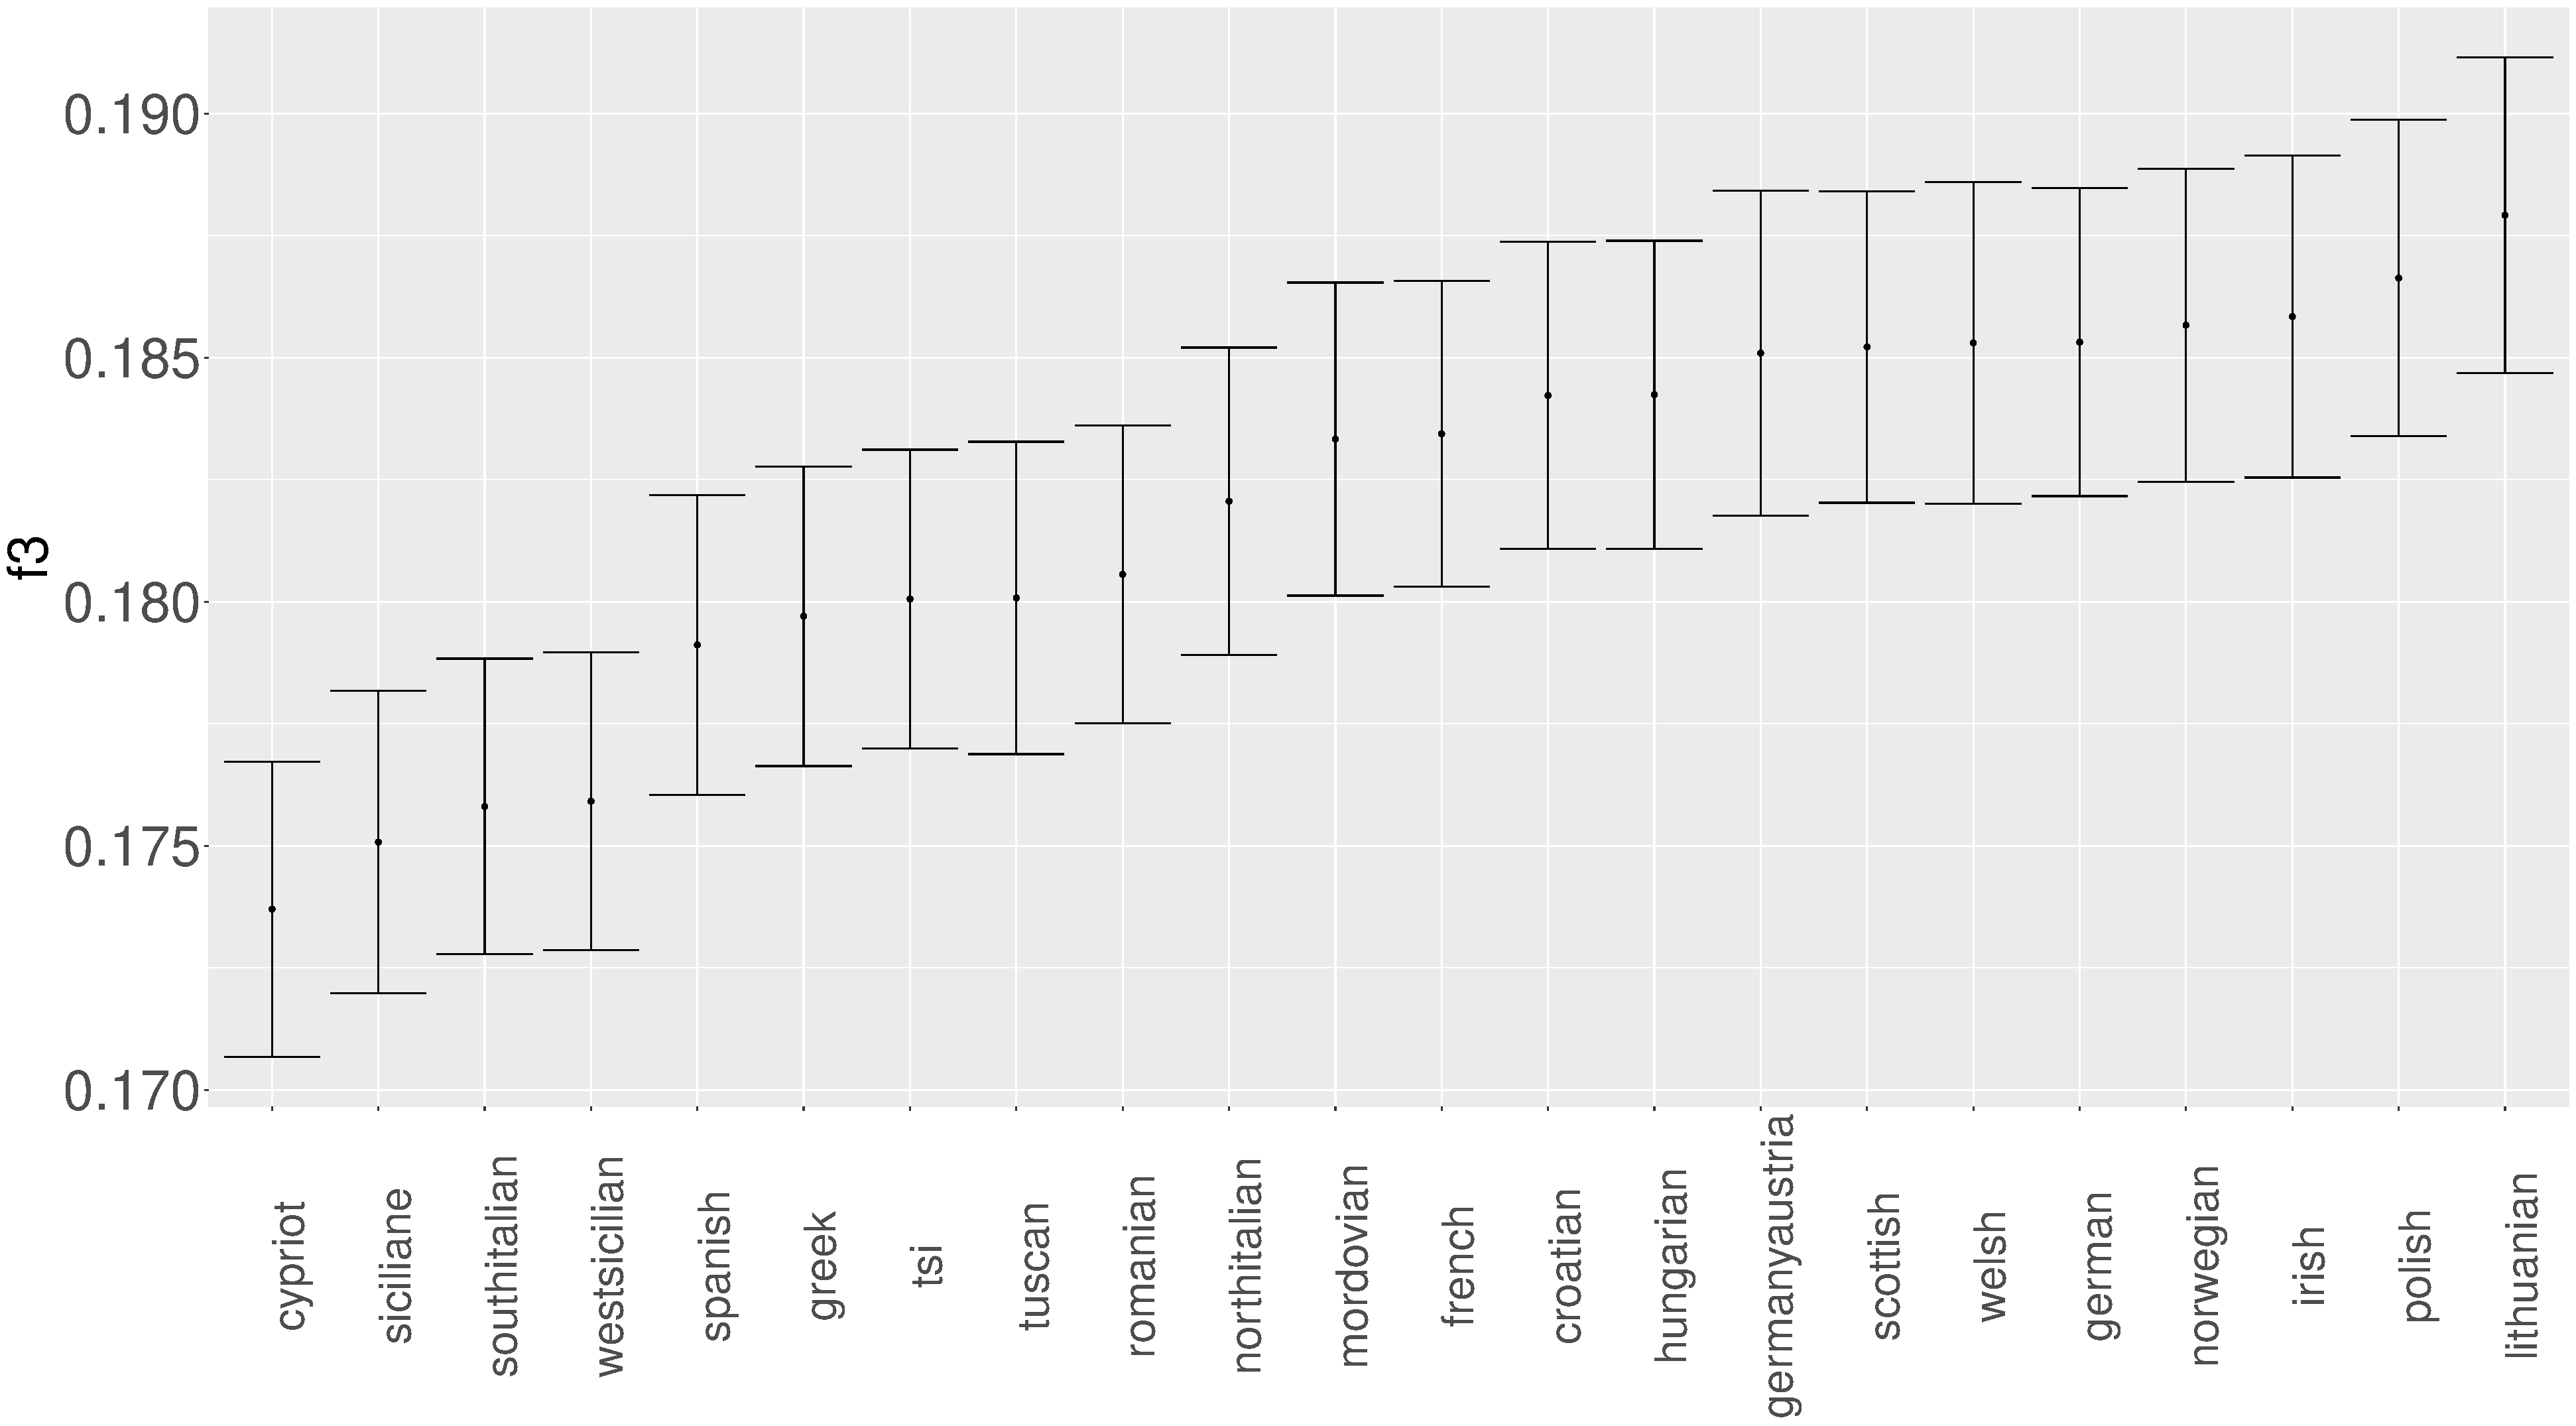
\includegraphics[width=1.0\textwidth]{../images/chapter5/f3_HB_ancient_slavs.pdf}
    \caption{$f_{3}$ statistics in the form of $f_{3}(EMA, present-day;mbuti pygmy$), where \textit{present-day} is different present-day European population. Error bars rerpesent $\pm*2$ standard error.}
    \label{fig:f3_HB_ancient_slavs}
\end{figure}


\subsection{Genetic structure and admixture events of present-day Slavic people}

fineSTRUCTURE clustering on the 17 ancient samples with 21 present-day European populations gave results similar to those obtained from visually inspecting the chunklengths matrix in Fig \ref{fig:copymatrix_moderns_ancient_slavs}. Among Migration Period samples, LIB2 and LIB12 cluster with north-west European groups, LIB3 clusters with Tuscany, and LIB4/LIB5 cluster with Spain. The present-day Slavic populations I had data for fall into two fineSTRUCTURE clades consistent with geography: (1) Croatians and Bulgarians (``south-east''), (2) Belarusians, Lithuanians, Polish, Russians and Ukrainians (``east''). Of the Early Middle Age samples, three (POH3, POH39, POH27) cluster into `south-east' Slavic clade, with the remaining seven clustering into the `east' clade. These results are consistent with the a hypothesis that the structure in present-day Slavic populations has been present since the Early Middle Ages.


\begin{figure}[htp]
    \centering
    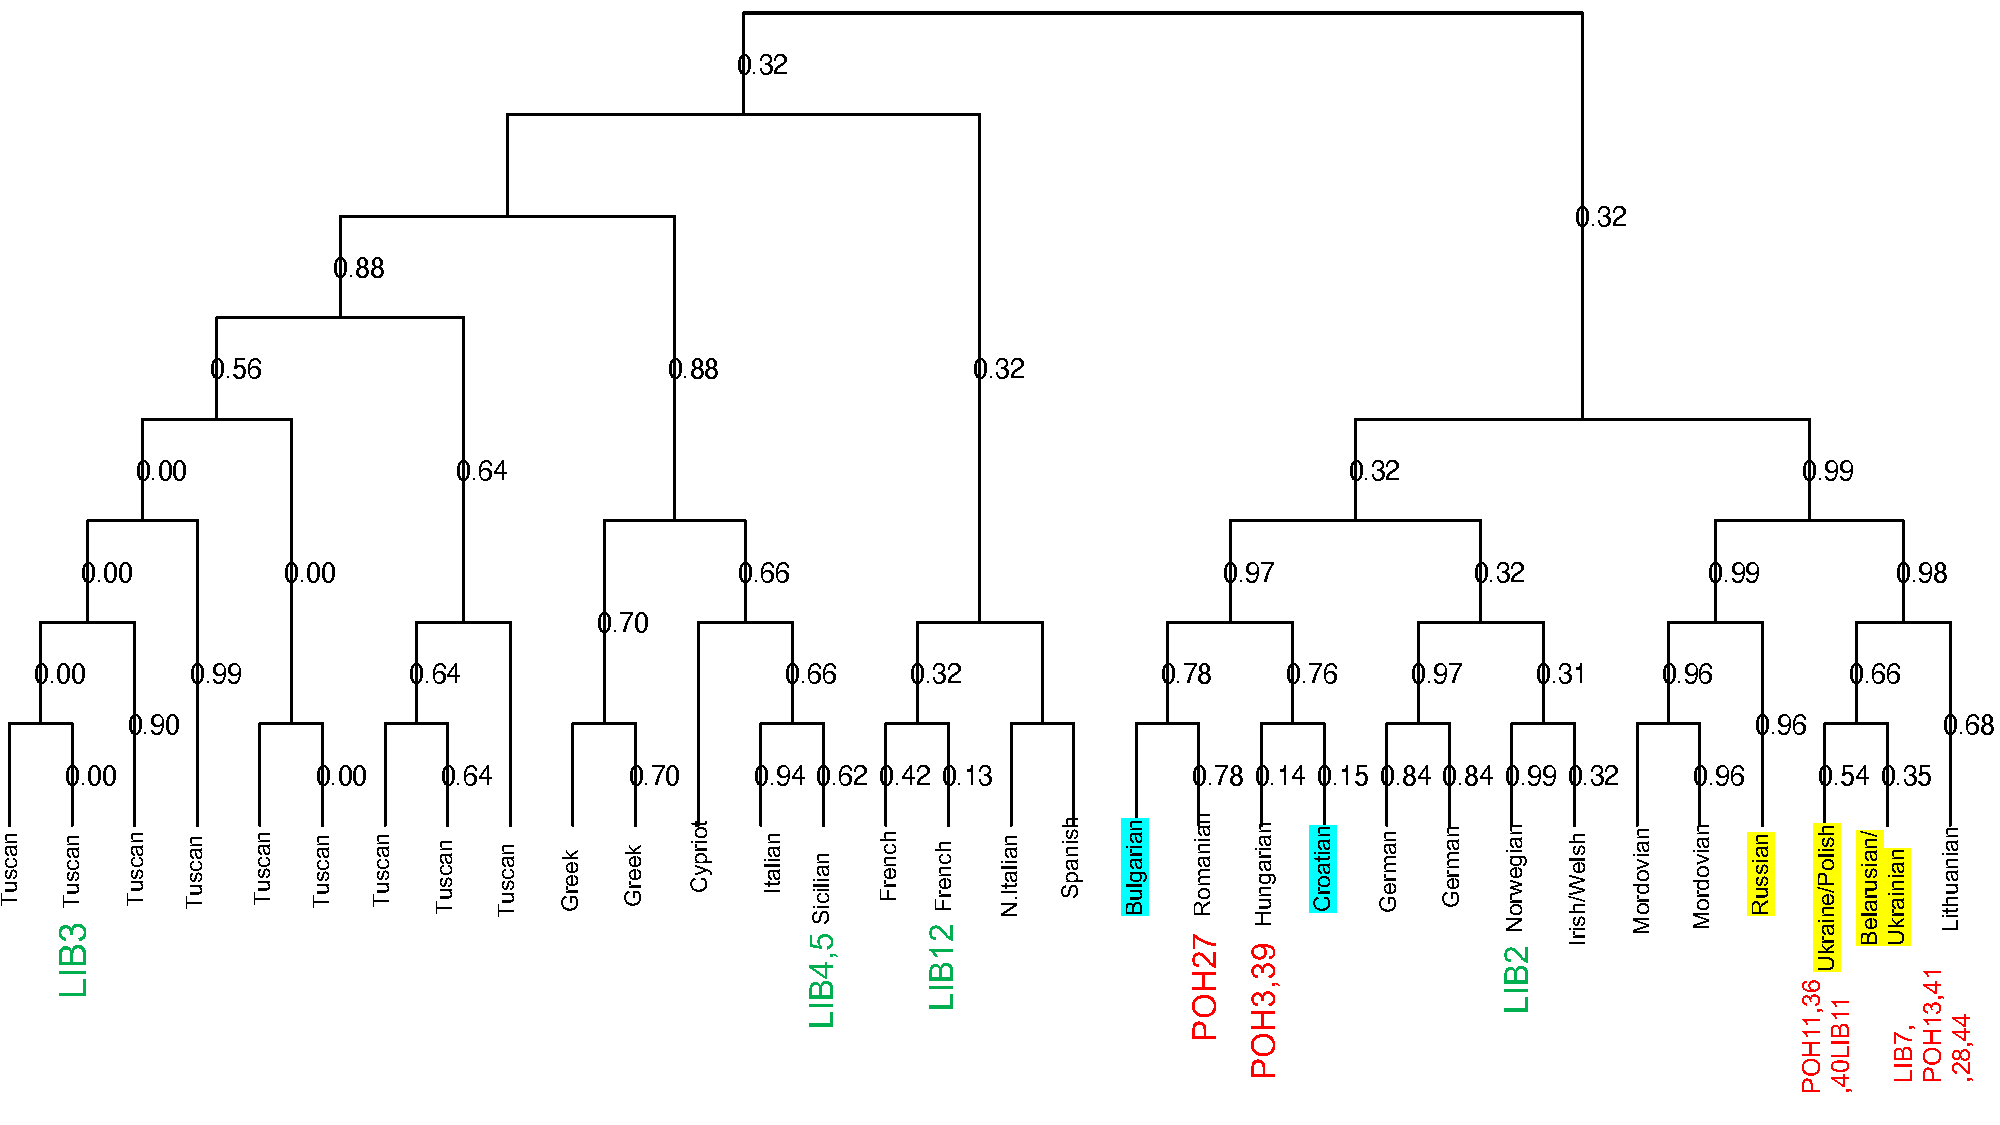
\includegraphics[width=1.0\textwidth]{../images/chapter5/tree_with_ancients.pdf}
    \caption{Population dendrogram generated by the fineSTRUCTURE tree building algorithm. Labeled tips refer to the primary population(s) represented in that clade. present-day non-Slavic populations shown in black. `south-east' Slavs highlighted in cyan and `north-west' Slavs highlighted in yellow. Migration period individuals superimposed in green and Early Middle Age samples superimposed in red. Read fineSTRUCTURE paper for description of edge values. Note: some tips contained more than one population but were not included as labels to save space.}
    \label{fig:tree_with_ancients}
\end{figure} 


Previous studies have identified admixture events in present-day Slavic populations involving an east-Asian source approximately 440 - 1080 CE \cite{Hellenthal2016, MOSAIC_2019}. In previous sections, I showed that this signal exists in the Early Middle Age ancient samples and is best characterised by populations from present-day Mongolia (Fig. \ref{fig:EarlyMiddleAges_MOSAIC_3way_moderns_Mu}). I employed MOSAIC \cite{MOSAIC_2019} to replicate the results of Hellenthal et al (2014) and Myers and Salter-Townshend (2019) and determine whether a similar admixing source is present in the ancient populations. I analysed all present-day populations (Table \ref{tab:MOSAIC_pops_slav}) and ancient Slavic populations in turn. For the ancient Slavic samples, I grouped all Early Middle Age samples together and grouped LIB3, LIB4 AND LIB5 together as the Migration Period samples. 

When considering 2-way admixture event, all of the tested populations (both ancient and present-day), bar the Migration Period, showed evidence of an admixture event involving a minor source that has the lowest $f_{st}$ with present-day Uygurs. The dates and bootstrapped confidence intervals are given in Fig. \ref{fig:MOSAIC_admixture_dates_plot}. Other than Norwegians and Croatians, whose dates are later and earlier respectively, the dates for other populations appear to be constrained around 1250 CE. This date is similar, but slightly later than that obtained from Hellenthal et al (2014), who estimate it to be 440 to 1080 CE.

\begin{figure}[htp]
    \centering
    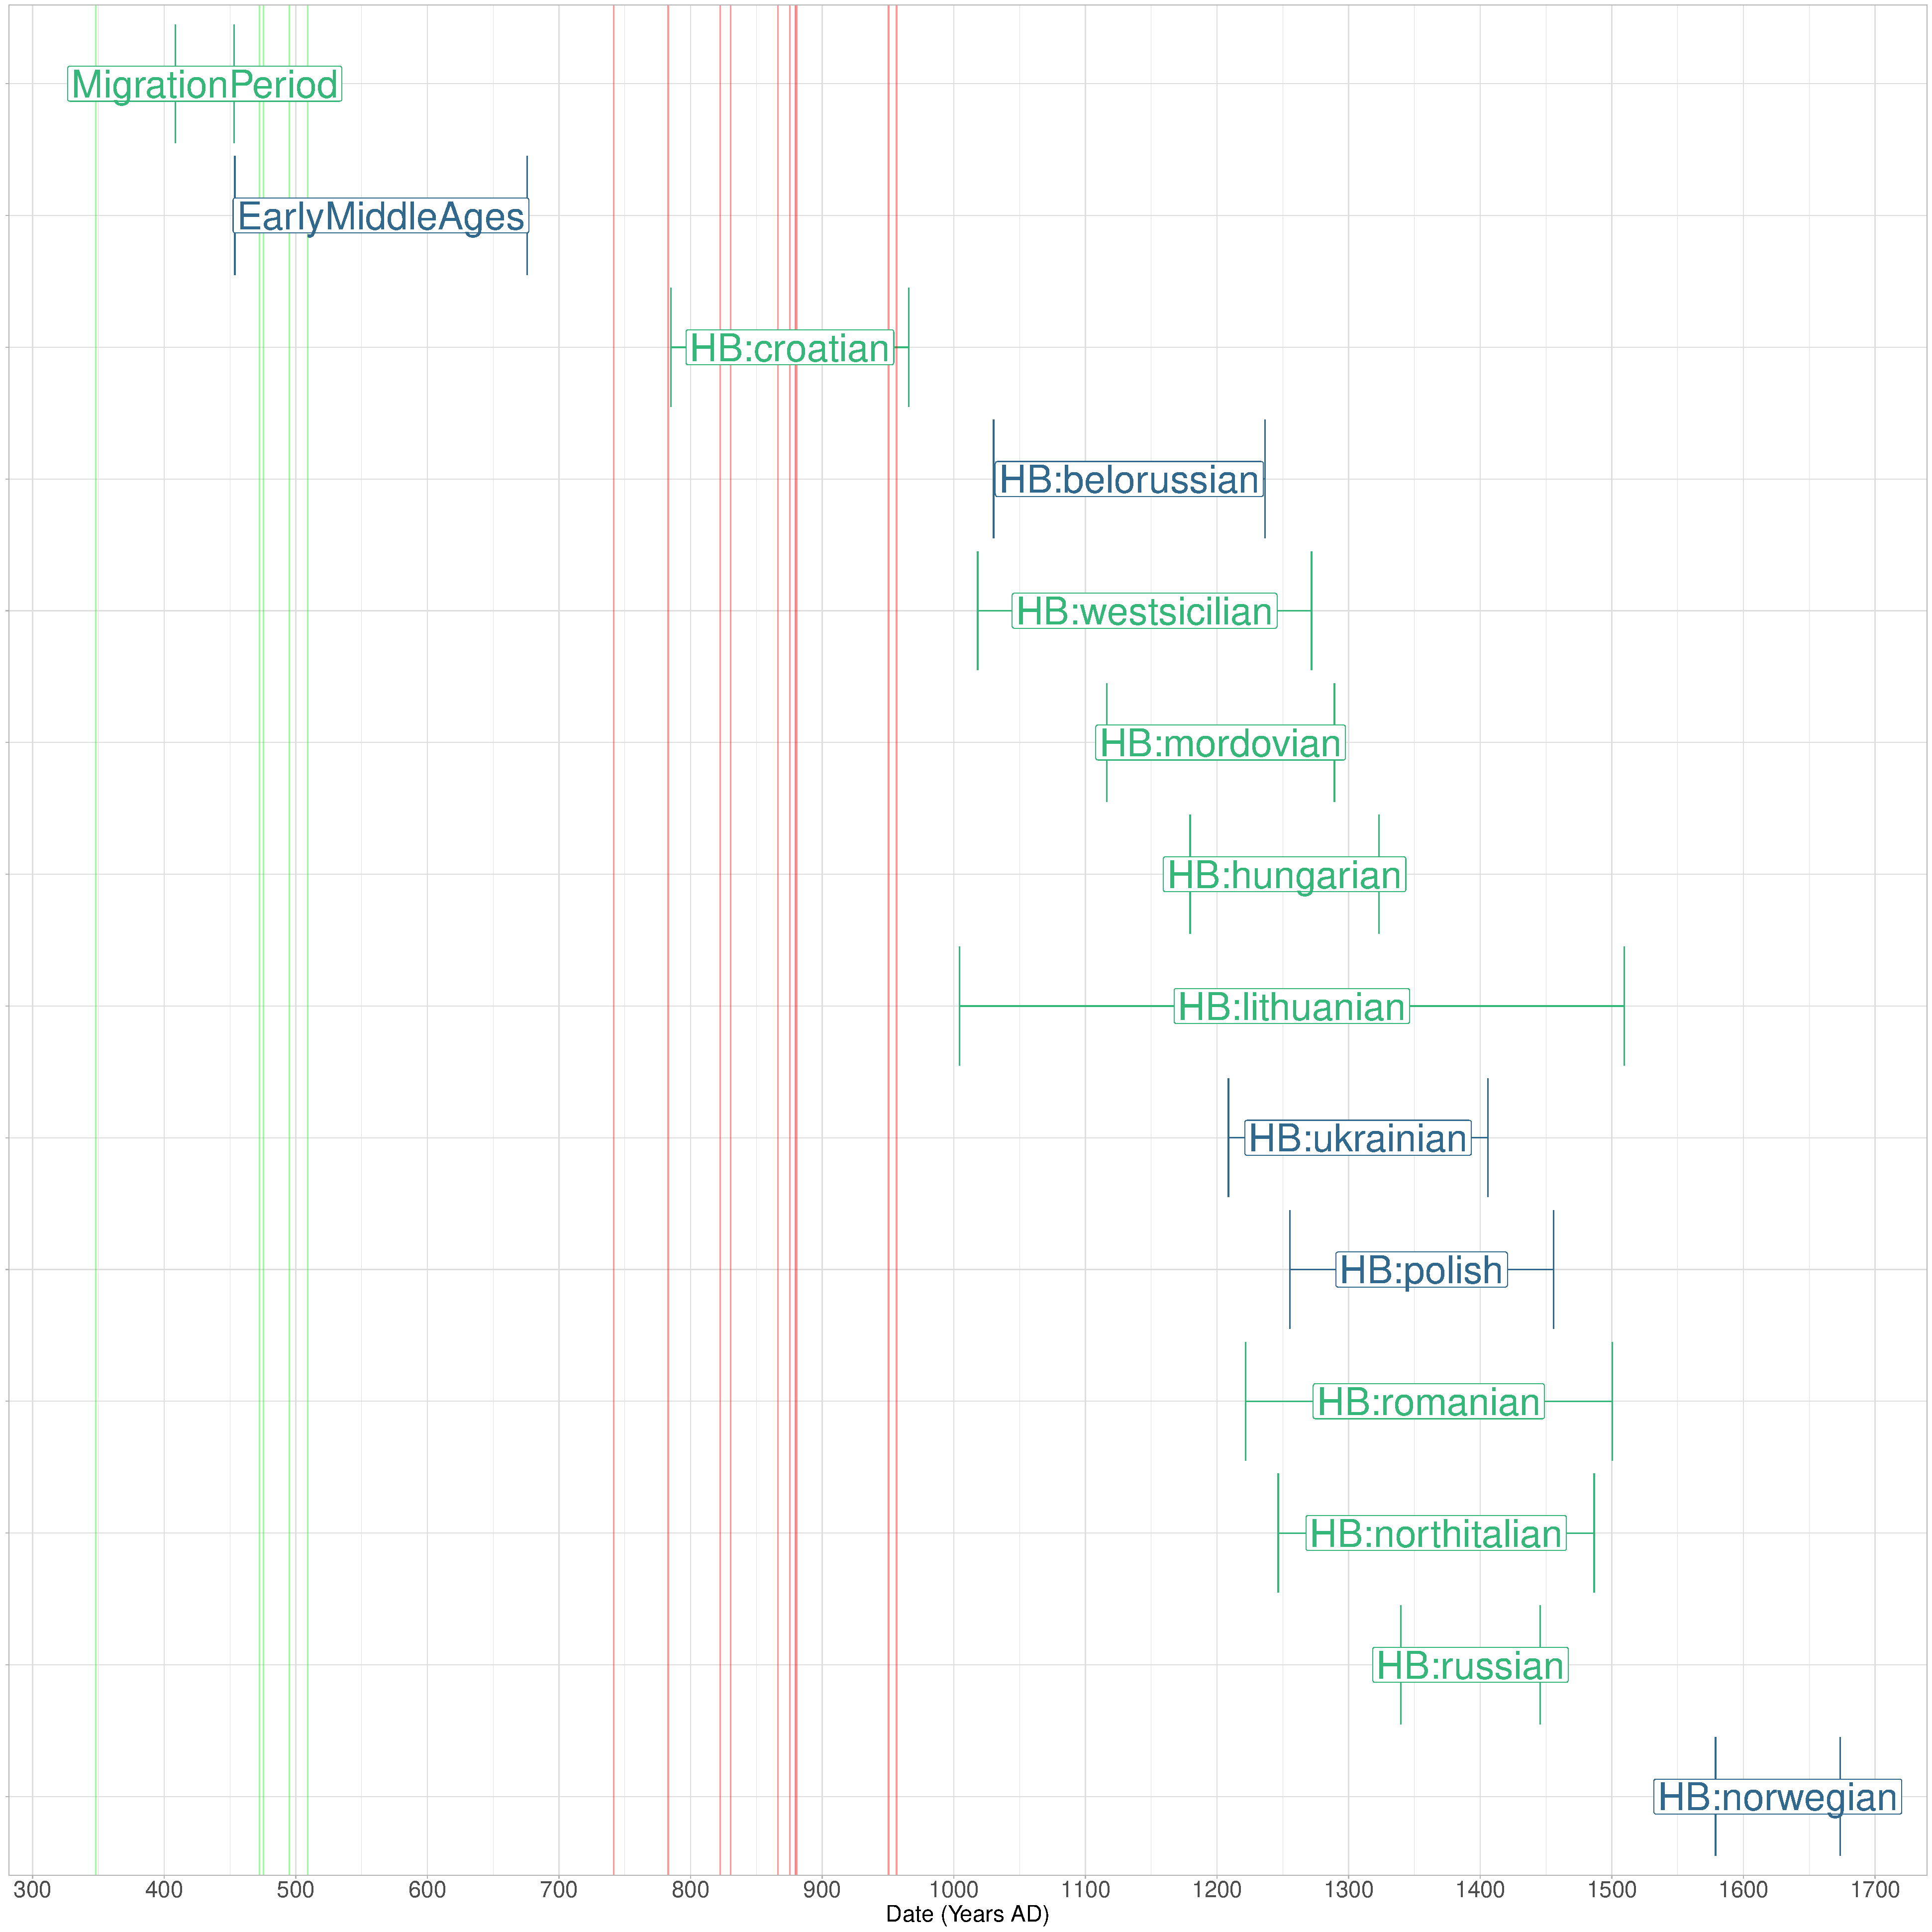
\includegraphics[width=1.0\textwidth]{../images/chapter5/MOSAIC_admixture_dates_plot.pdf}
    \caption{MOSAIC inferred 2-way admixture dates with bootstrapped 97.5\% and 2.5\% CI. Vertical green lines correspond to radiocarbon estimated dates of Migration Period samples and red lines equivalent for Early Middle Age samples. Estimated dates obtained by assuming an average generation time of 26 and date of birth of 1950 for present-day samples.}
    \label{fig:MOSAIC_admixture_dates_plot}
\end{figure} 

Of the present-day Slavic speaking populations, Belorussian, Polish and Ukrainian, show evidence of a 3-way admixture event, in which the middle component has the lowest $f_{st}$ with Migration Era ancient samples (Fig. \ref{fig:Fst_plot_HB:lithuanian}). The major component has a low $f_{st}$ with Early Middle Age Slavs. This suggests that the formation of present-day Slavic populations could have occurred via admixture events involving Migration Era individuals with high levels of Southern European ancestry, Middle Age Era samples which show a strong affinity to present day eastern Europeans, and a small but significant east Asian source best represented by present-day Uygurs. These results are similar to those in the Middle Age samples (Fig. \ref{fig:EarlyMiddleAges_MOSAIC_3way_moderns_Mu}), though dates are more recent in the present-day samples (Fig \ref{fig:MOSAIC_admixture_dates_plot}), suggesting recent admixture in present-day populations may be masking the older signals we see in the Early Middle Ages group.

\begin{figure}[htp]
    \centering
    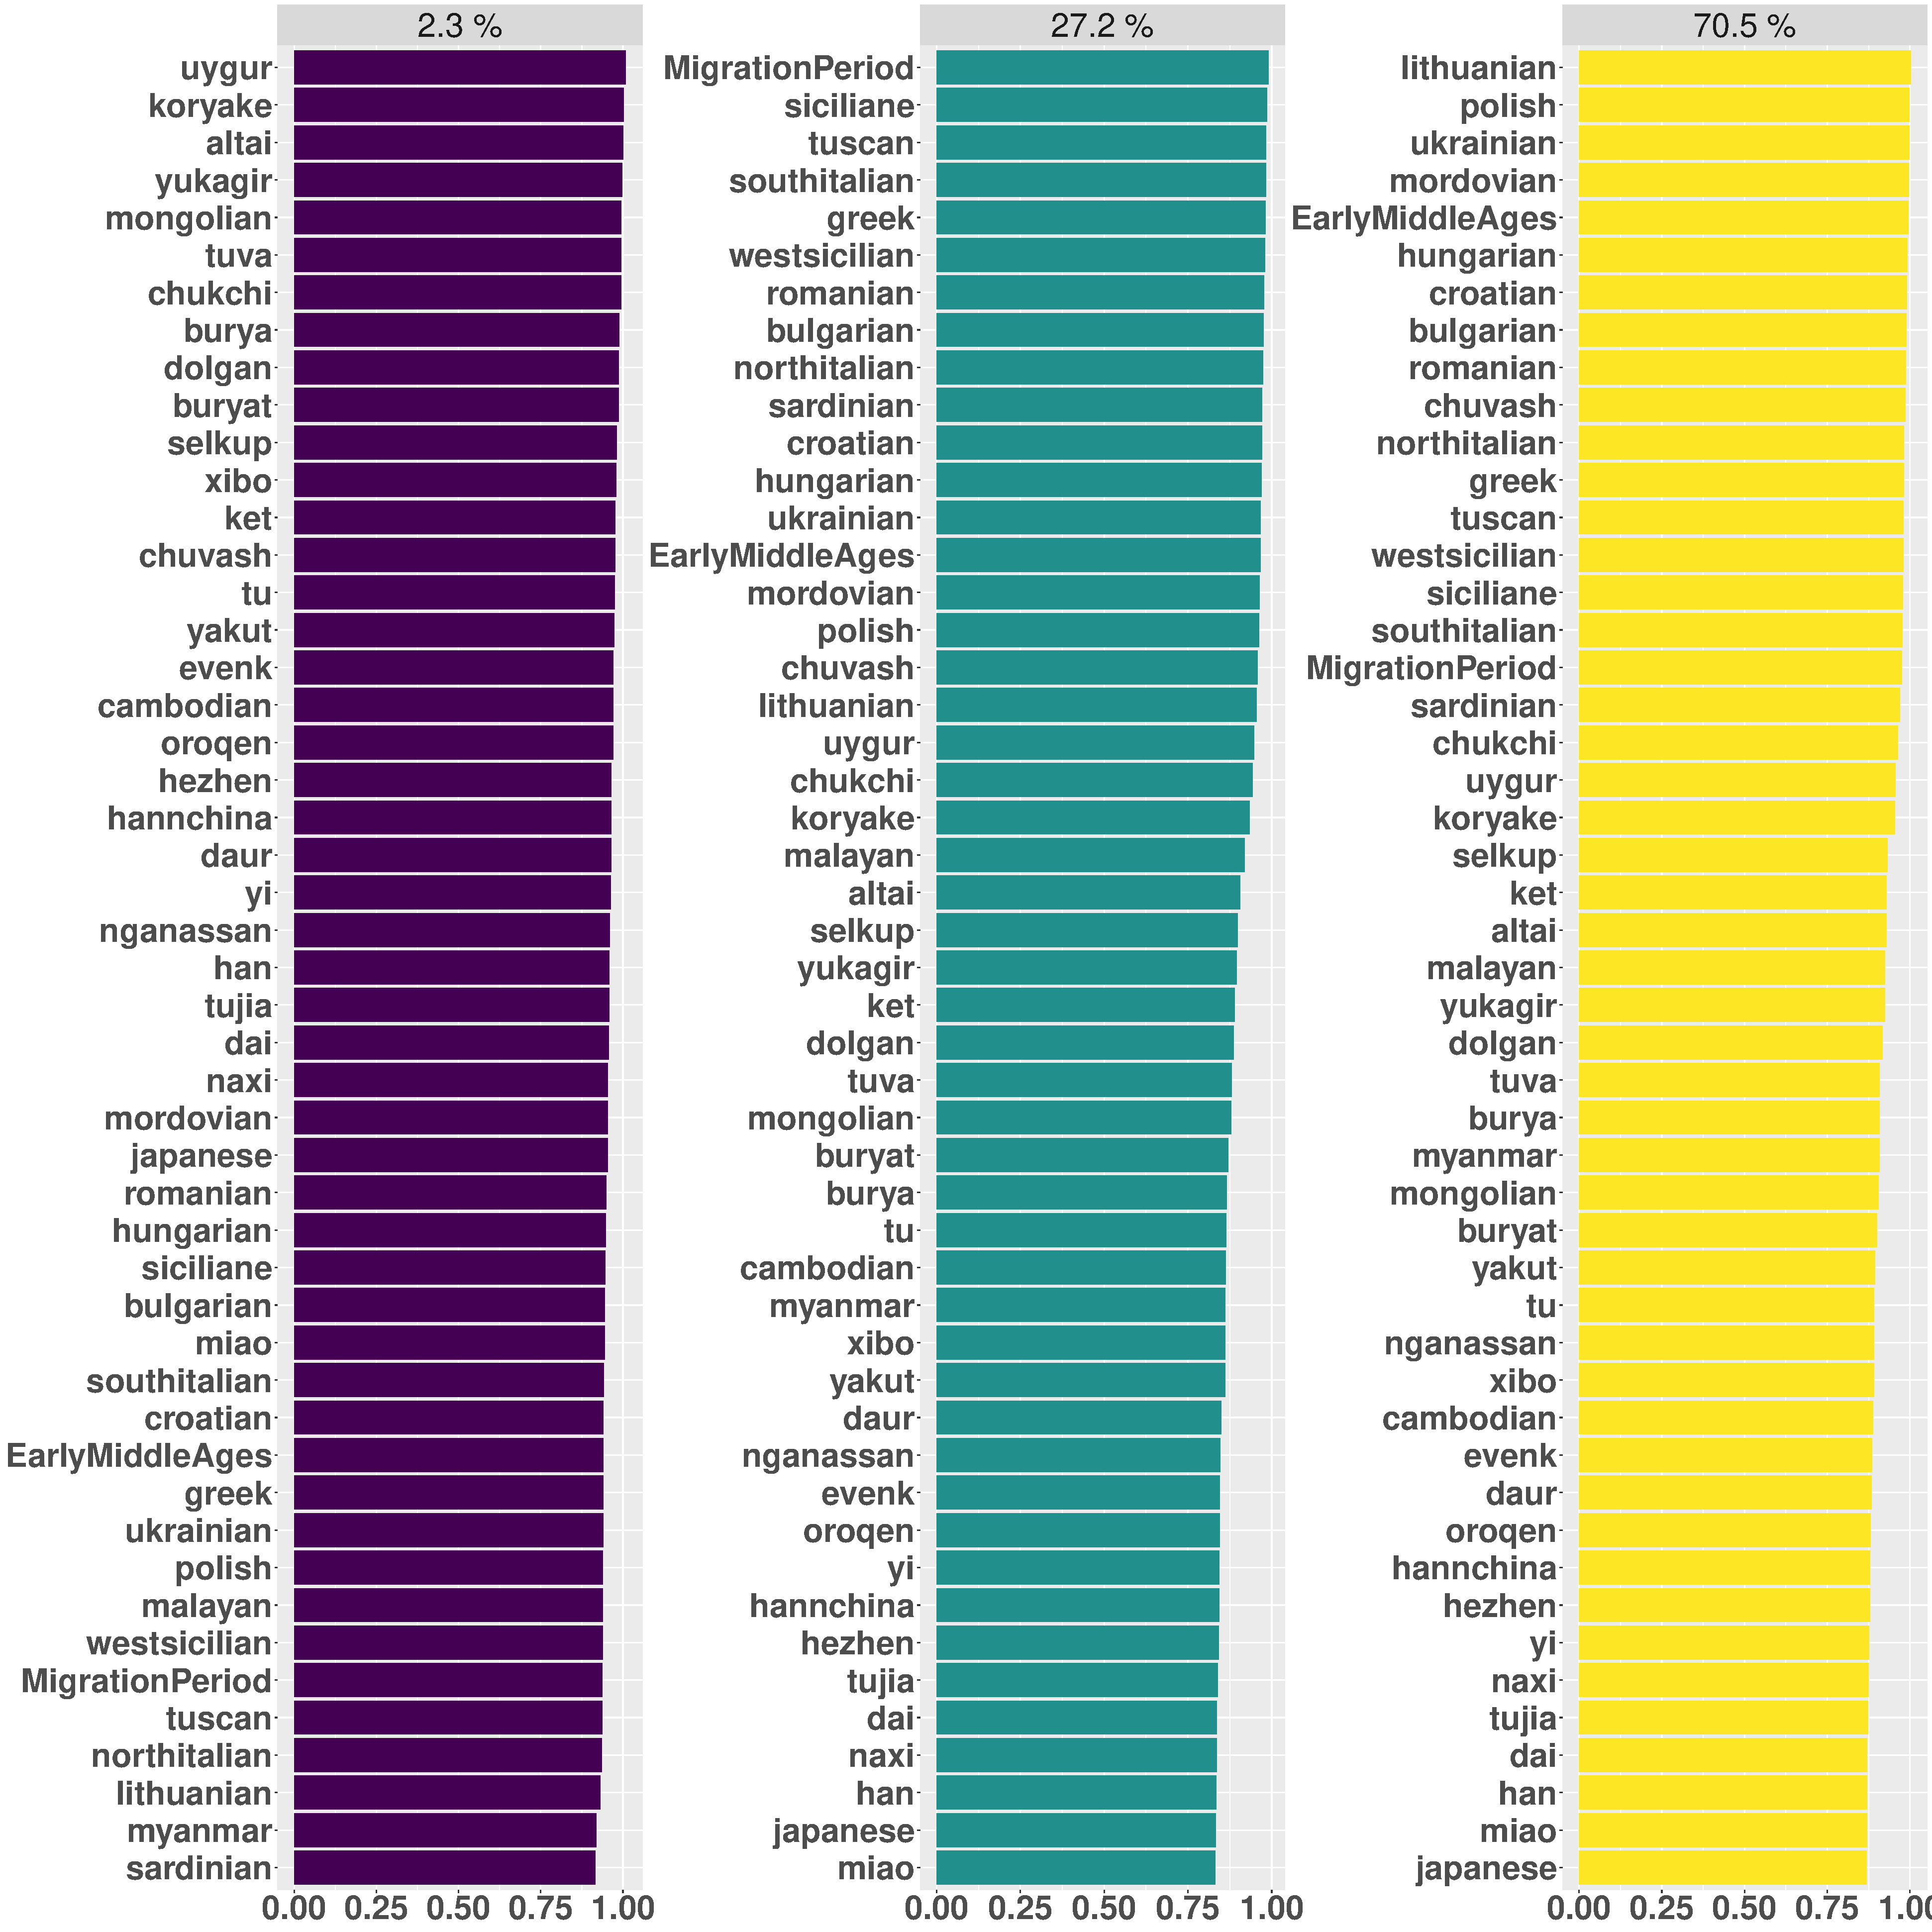
\includegraphics[width=1.0\textwidth]{../images/chapter5/Fst_plot_HB:belorussian.pdf}
    \caption{$1 - F_{st}$ between 3 inferred mixing sources for present-day Belorussians. Each panel represent a different mixing source. Each bar gives the value $1-F_{st}$ between that samples population and the mixing source. Higher values of $1-F_{st}$ suggest that source is well represented by a particular population. }
    \label{fig:Fst_plot_HB:lithuanian}
\end{figure} 

\section{Summary of Results and Discussion}

Referring back to the questions posed in the introduction.

I found that the Migration Period samples, relative to the Early Middle Age samples, show a high degree of diversity in terms of ancestry, with affinities to present-day samples varying from Norway to southern Italy. On the other hand, fineSTRUCTURE analysis on the `ancients' painting grouped all Early Middle Age samples together, showing that they represent a group of samples which likely share common ancestry. Consistent with this, the Early Middle Age samples showed evidence of east Asian admixture, a signal that was not present in the Migration Period samples. These results suggest a population turnover may have occurred between approximately 500-700 AD, the time period between the Migration Period and Early Middle Age. However, based on MOSAIC results of present day populations, a model of mixture between sources close to Migration Era, Early Middle Age and east-Asians seems plausible (Fig. \ref{fig:Fst_plot_HB:lithuanian}).


All of the Early Middle Age samples showed a high genetic similarity to present-day Slavic and non-Slavic speaking populations from eastern Europe, such as Poland and Lithuania (Fig. \ref{fig:copymatrix_moderns_ancient_slavs}). This is in stark contrast to the Migration Period, who all fell on a cline of genetic similarity between present-day Scandinavian and Mediterranean populations (Fig. \ref{fig:chunklengths_moderns_ancients_PCA}). These results provide strong evidence that continuity exists between the Early Middle Ages and the present-day, but not between the Migration Period and Early Middle Ages.

Finally, a joint fineSTRUCTURE analysis which included both ancient and present-day samples showed that present-day Slavic speakers can be split into  `north-west' and `south-east' groups, and that different Early Middle Ages samples had differing affinities to these groups (Fig \ref{fig:tree_with_ancients}). 

I found strong evidence that LIB2 was a recent migrant from Viking regions. There are many sources which detail the links between the Viking and Slavic peoples towards the end of the first millennium \cite{duczko2004viking, peterson2016vikings}. However, most evidence suggests these links occurred later than the estimated radiocarbon date of LIB2. For example, it is known that the Scandinavian colonists settled in present-day Russia as early as 750 AD, whilst LIB2 was samples at approximately 495 AD. Therefore, we could suggest that this is evidence of an earlier link than previously known. In their large-scale study of ancient DNA of Viking samples from across Europe, Margaryan et al (2020) present Viking samples and ancestry in Estonia, but not until the beginning of the 8th Century, some 200 years after the estimated date of LIB2.  

I also found evidence of southern European-like ancestry in three (LIB3, LIB4 and LIB5) Migration Period samples. The appearance of southern European-like ancestry in Central Europe in the first millennium is similar to a signal found in a study exploring the ancestry of individuals with elongated skulls in medieval Bavaria (approximately 500AD) \cite{Veeramah2018}. It was shown that particular individuals harbour substantial Southern-European ancestry from outside of Bavaria, closest to individuals from present-day Greece and Turkey. There are at least two possible explanations for the presence of this ancestry in the Migration Era samples. Firstly, LIB3, LIB4 and LIB5 may be similar migrants to the region. This is consistent with the fact they are all female; Veeramah et al (2018) showed that there was a tendency for females to migrate from southern regions, perhaps related to the formation of strategic alliances. Alternatively, it is possible these individuals are a leftover from a historically described Lombard migration that moved from Northern Germany through Czechia, Slovakia, Hungary and ended up in Lombardia (Z. Hofmanova, personal communication). Accordingly, this could appear as genetic similarity to present-day populations from Northern Italy. This hypothesis is supported by the clustering of LIB3, LIB4 and LIB5 with present-day Italian samples in the `present-day' fineSTRUCTURE analysis (Fig \ref{fig:tree_with_ancients}).

The results from the analysis of combined ancient and present-day genomes are consistent with those from Kushniarevich et al (2015) \cite{Kushniarevich23015} who determined that Eastern (Russia, Belarus, Ukraine) and Western (Polish) central European Slavs form a cluster to the exclusion of Southern Slavs (Croatia, Bulgaria), whilst also remaining distinct from geographically proximate Germanic (German/Austrian) and Baltic (Lithuanian) populations. This is also consistent with results from Veeramah et al 2011, who showed that Sorbs, a west-Slavic population found between Poland and Germany, have a much stronger affinity to more distant Slavic populations from Czechia than to more proximate Germans \cite{veeramah2011genetic}. 

